\chapter[\leavevmode\newline Differential cross-section of $B^0_s \to J/\psi \phi$]{Differential cross-section of $B^0_s \to J/\psi \phi$}
\chaptermark{Differential cross-section of $B^0_s \to J/\psi \phi$}
\label{chap:Chapter_5}

\section{Total efficiency}

The acceptance $\alpha$ is defined as the ratio of the number of $B^0_s$ mesons that meet the filter criteria for the kaons and muons candidates to the total number of $B^0_s$ mesons created in the MC simulation,

\begin{equation}
\alpha(p_T, |y|) = \frac{N(B^0_s; \ p_T, |y| ; \ \mathrm{filter \ criteria})}{N(B^0_s; \ p_T, |y| )}
\end{equation}

This value depends on the desired region for both $p_T$ and $|y|$. Because this manuscript takes into account several bins for these variables, a separate acceptance is obtained for each bin, as well as a total acceptance for the entire region. 

The reconstruction efficiency, $\epsilon$, is defined as the ratio of the number of $B^0_s$ mesons that meet all of the selection criteria from table \ref{table:sel_criteria} to the number of $B^0_s$ mesons that meet the filter criteria for kaons and muons candidates (the numerator of acceptance),

\begin{equation}
	\epsilon(p_T, |y|) = \frac{N(B^0_s; \ p_T, |y| ; \ \mathrm{full \ selection \ criteria})}{N(B^0_s; \ p_T, |y| ; \ \mathrm{filter \ criteria})}
\end{equation}

The total efficiency $\alpha \cdot \epsilon$, is the fraction of the generated $B^0_s$ mesons that actually correspond to the required candidates for investigation, that is, the mesons that decay through the channel studied in this work,

\begin{equation}
	\alpha \cdot \epsilon = \frac{N(B^0_s; \ p_T, |y| ; \ \mathrm{full \ selection \ criteria})}{N(B^0_s; \ p_T, |y|)}
\end{equation}

Fig. \ref{fig:effy_ptbins} shows the acceptance, efficiency and total efficiency for the $p_T$ bins and Fig. for the $|y|$ bins. It is observed that for increasing $p_T$, all of the ratios increase as well. % and $|y|$ bins respectively. 

\begin{figure}[htp!]
	\centering
	\begin{subfigure}[b]{0.475\textwidth}
		\centering
		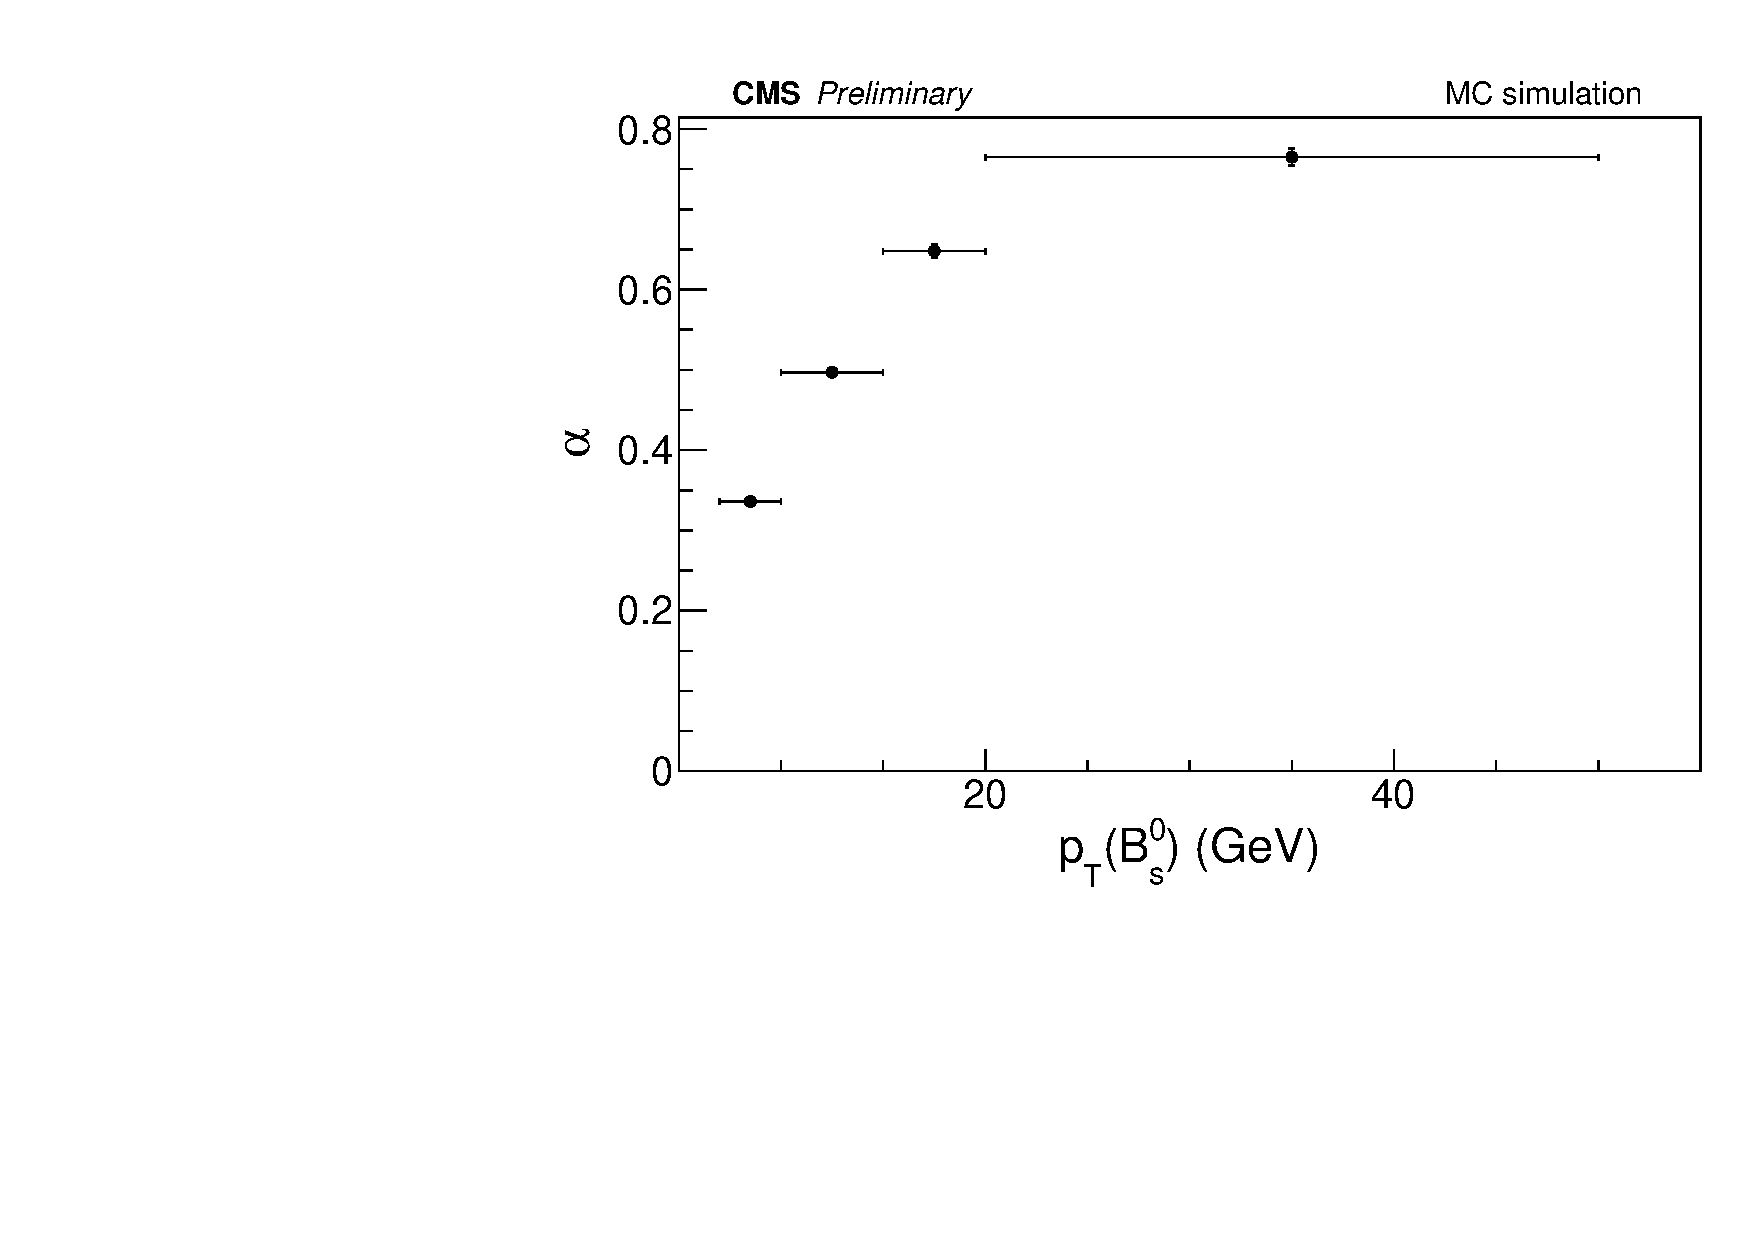
\includegraphics[width=\textwidth]{MainContent/Figs/effy/alpha_ptbins.PDF}
		\caption{}%
	\end{subfigure}
	\begin{subfigure}[b]{0.475\textwidth}
	\centering
	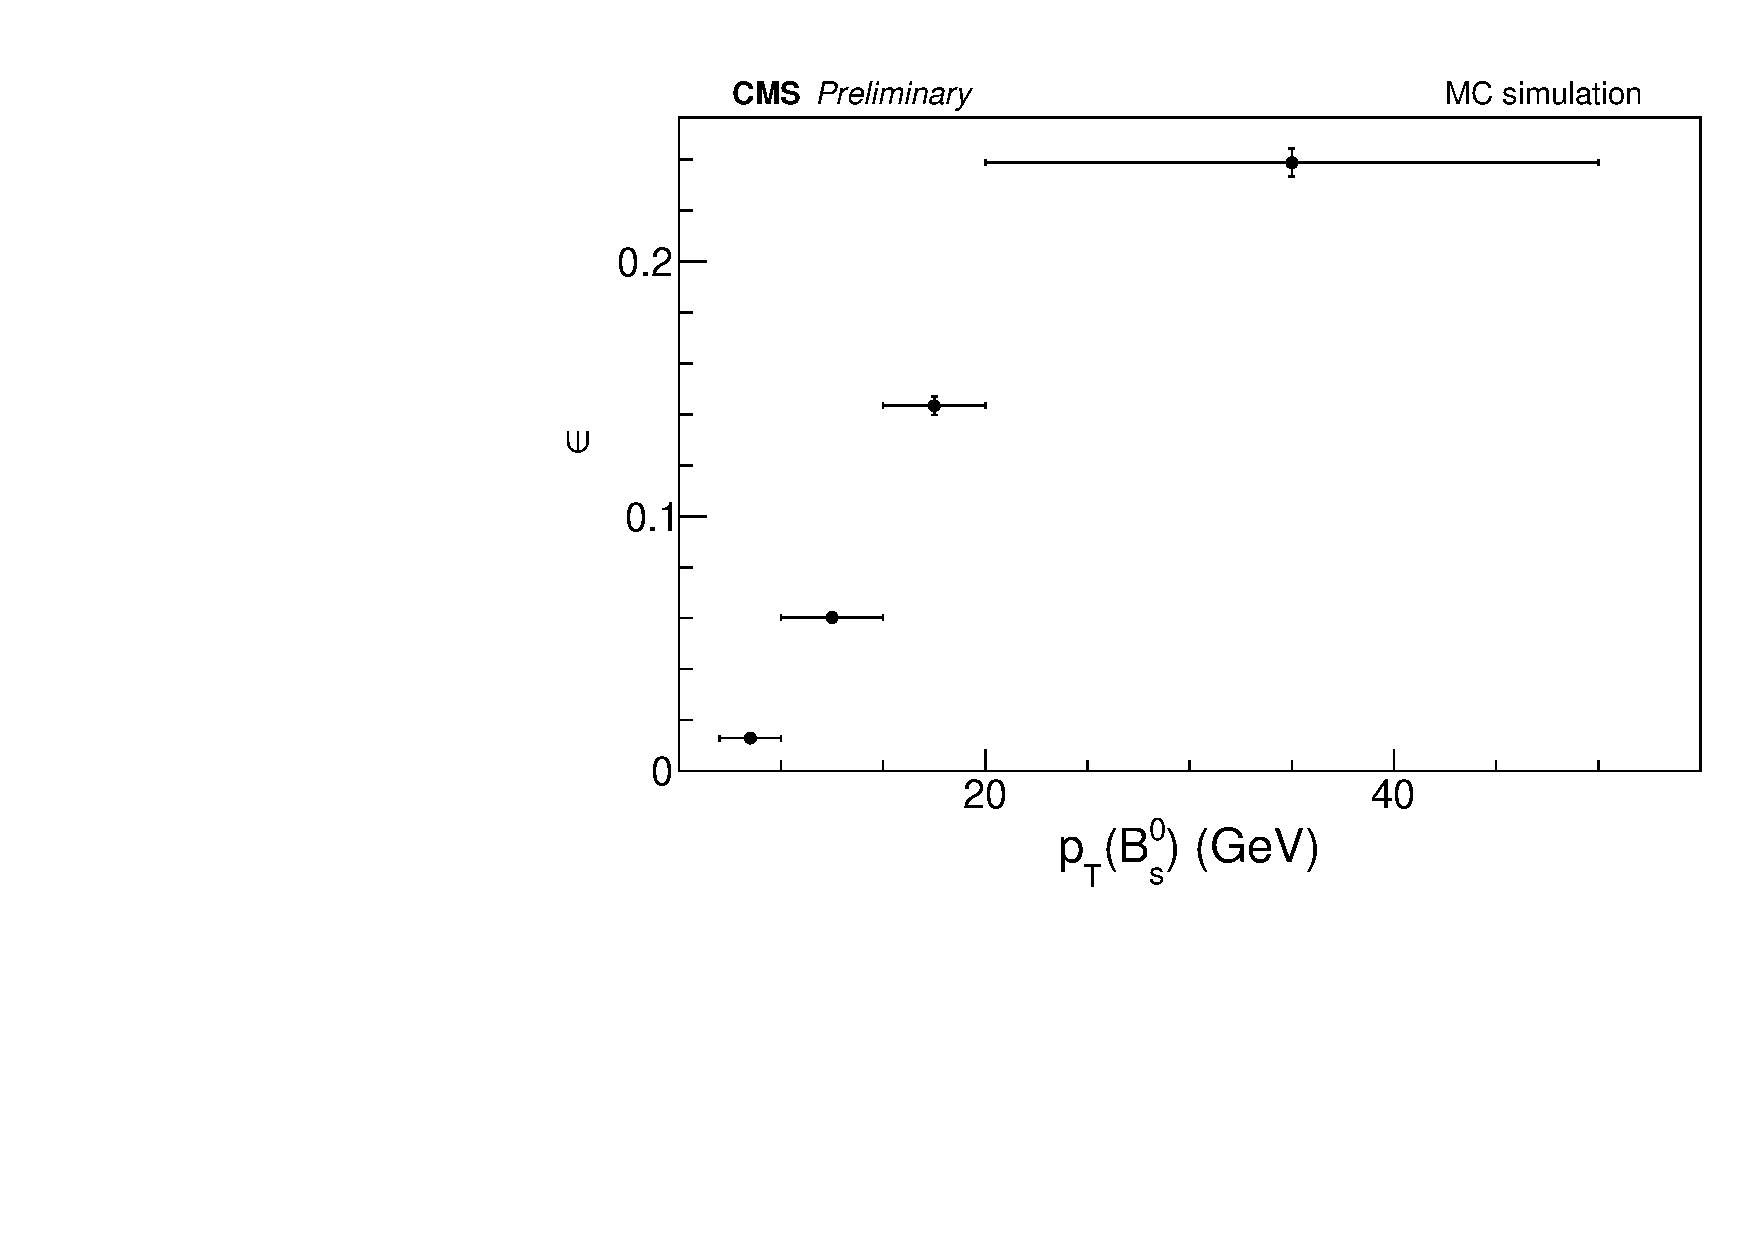
\includegraphics[width=\textwidth]{MainContent/Figs/effy/epsilon_ptbins.PDF}
	\caption{}%
\end{subfigure}
	\vskip\baselineskip
	\begin{subfigure}[b]{0.8\textwidth}
		\centering
		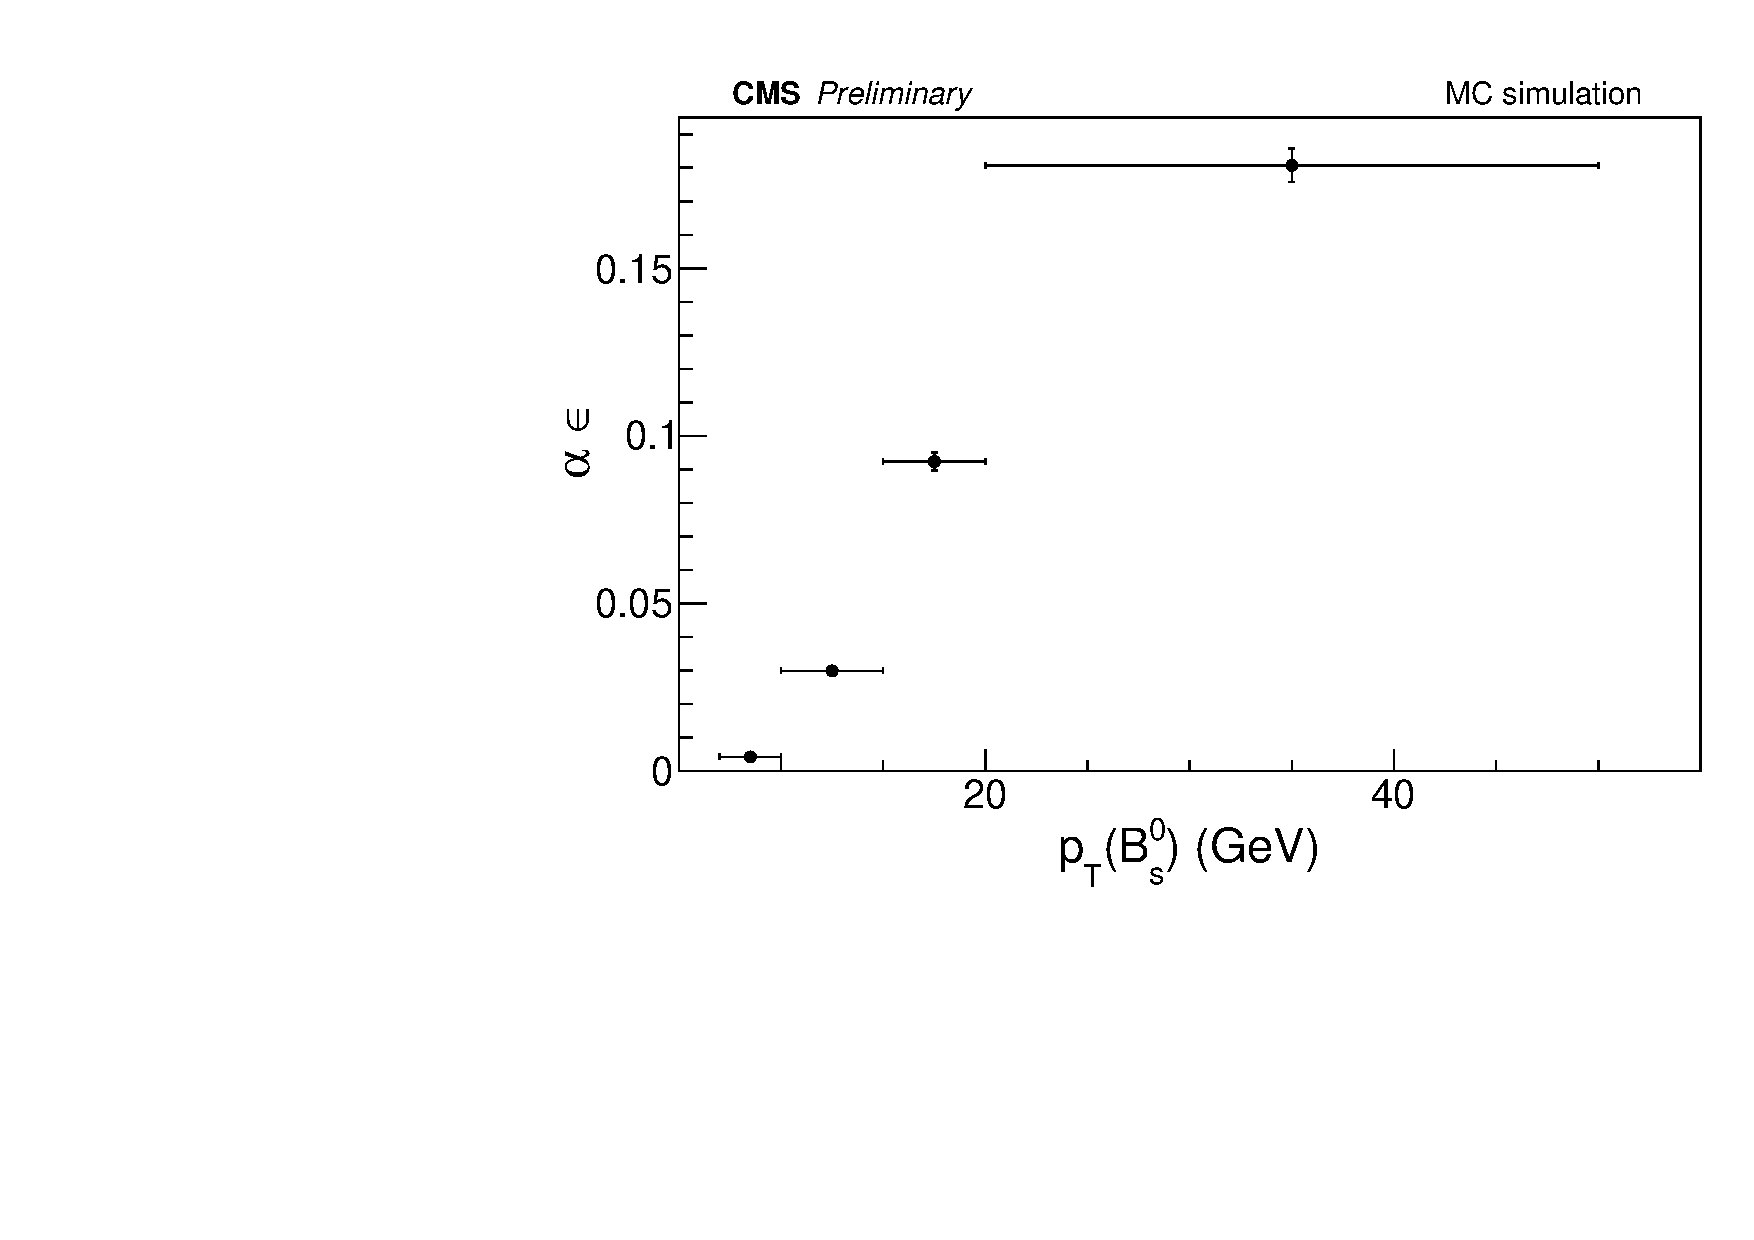
\includegraphics[width=\textwidth]{MainContent/Figs/effy/totaleffy_ptbins.PDF}
		\caption{}%
	\end{subfigure}
	\caption{(a) Acceptance, (b) efficiency and (c) total efficiency for the MC simulation using $p_T$ bins.}
	\label{fig:effy_ptbins}
\end{figure}

\begin{figure}[htp!]
	\centering
	\begin{subfigure}[b]{0.475\textwidth}
		\centering
		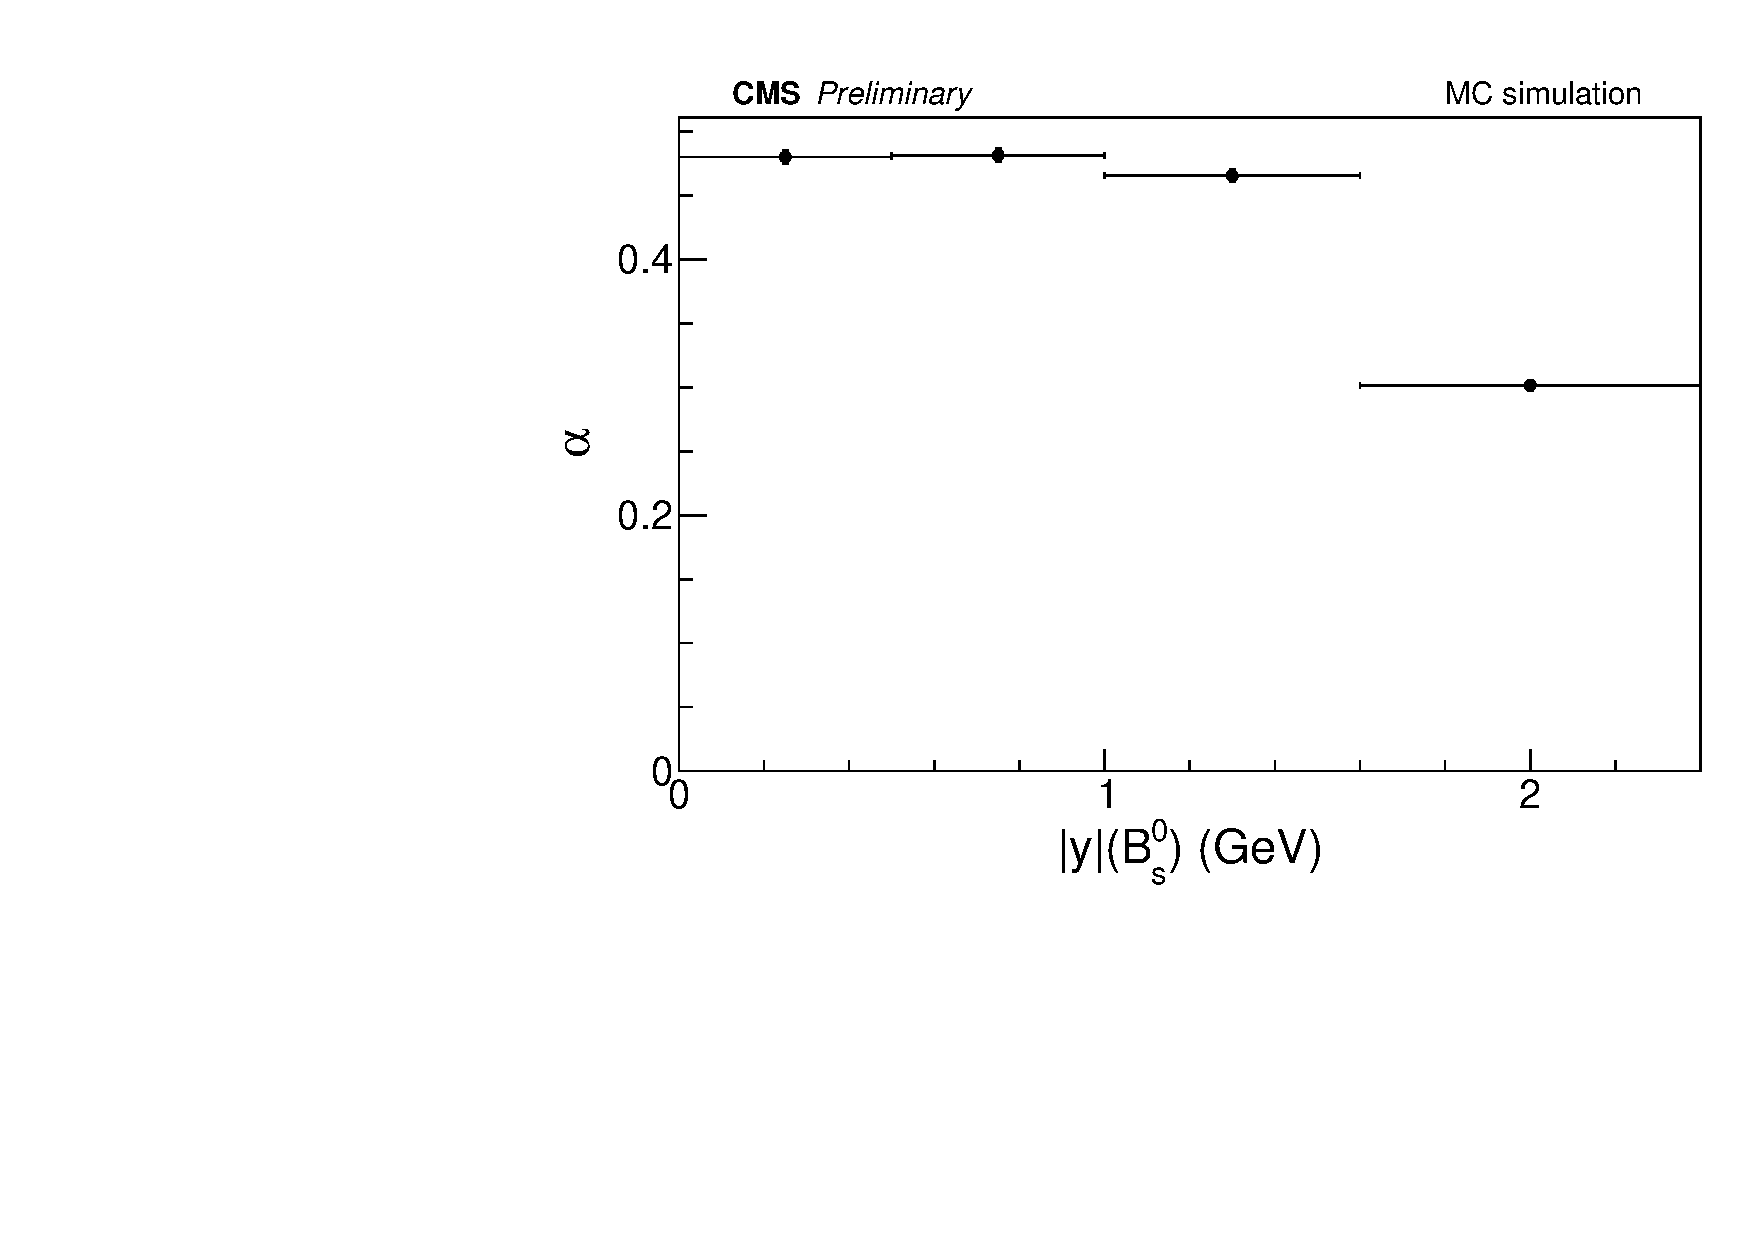
\includegraphics[width=\textwidth]{MainContent/Figs/effy/alpha_ybins.PDF}
		\caption{}%
	\end{subfigure}
	\begin{subfigure}[b]{0.475\textwidth}
		\centering
		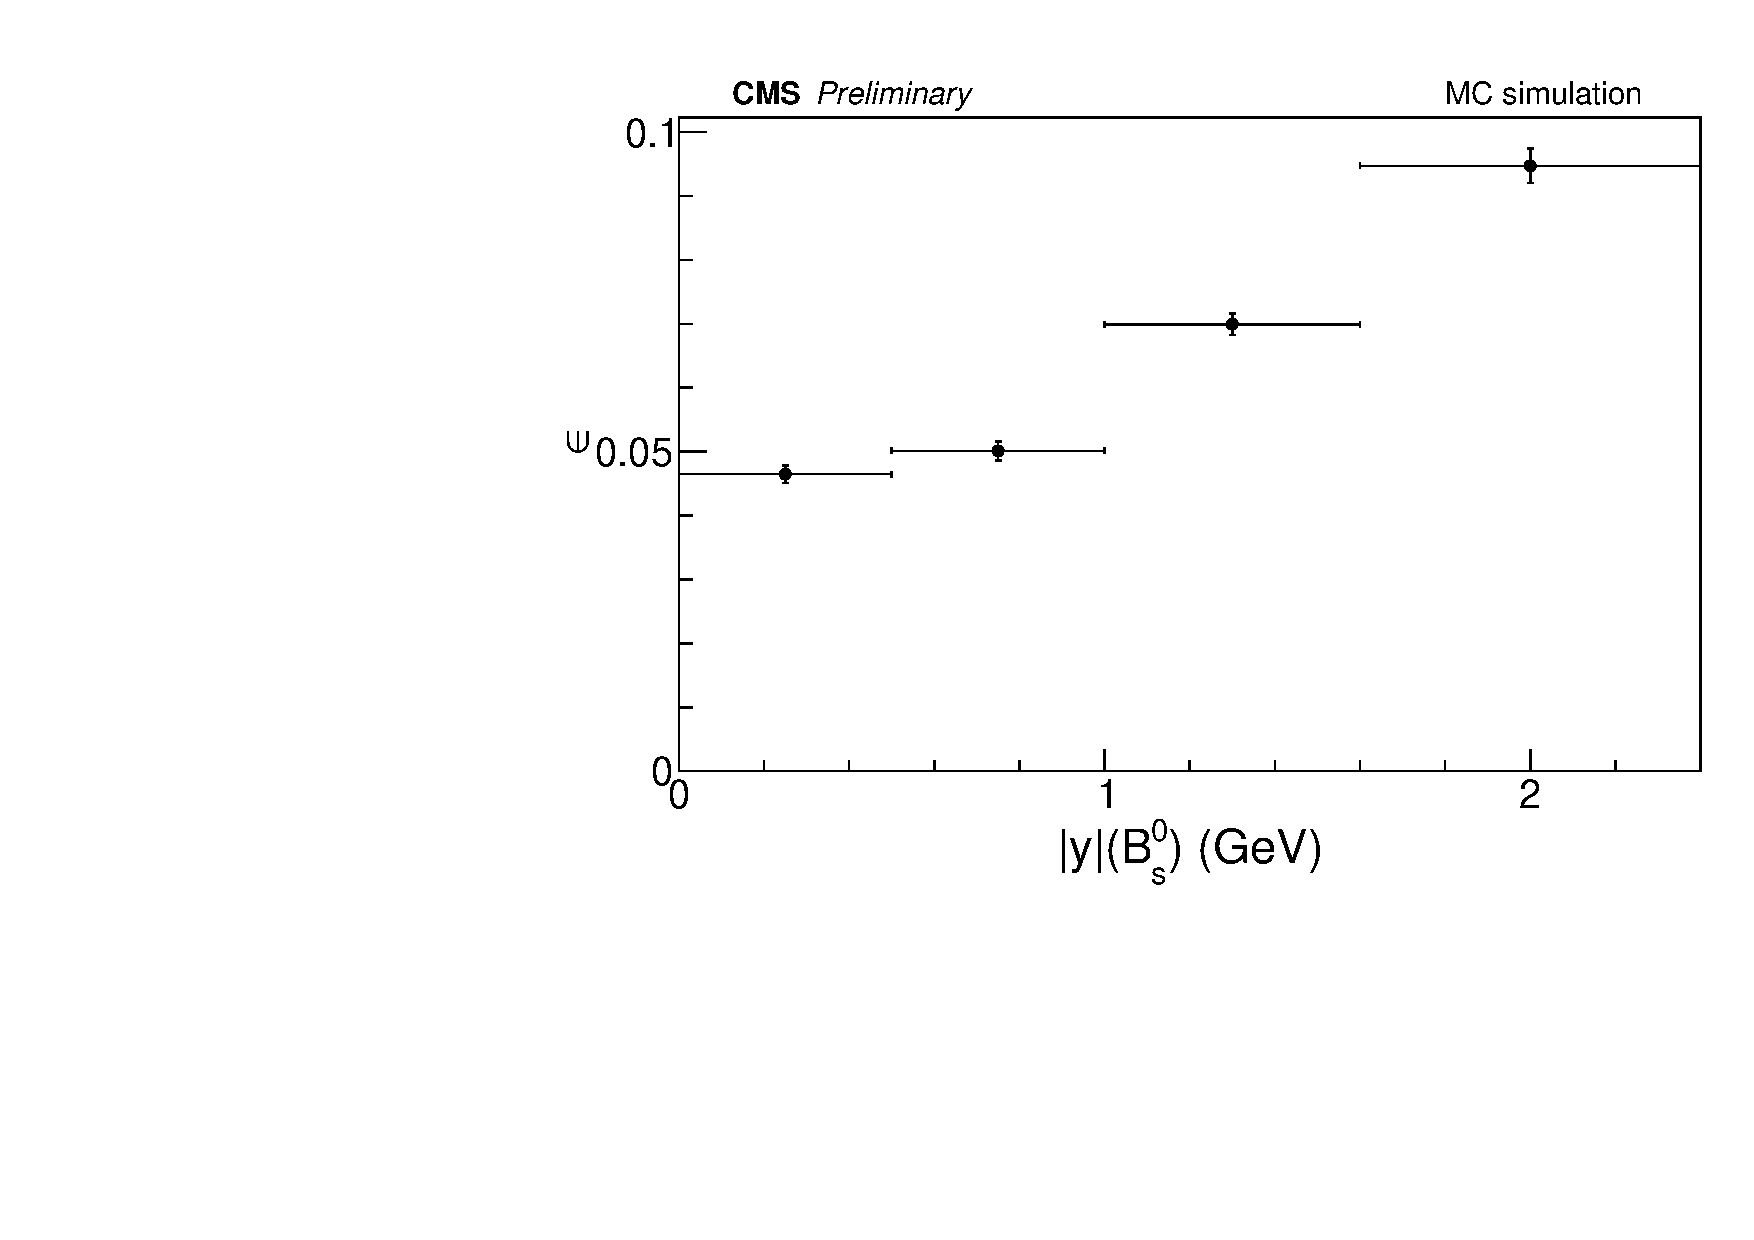
\includegraphics[width=\textwidth]{MainContent/Figs/effy/epsilon_ybins.PDF}
		\caption{}%
	\end{subfigure}
	\vskip\baselineskip
	\begin{subfigure}[b]{0.8\textwidth}
		\centering
		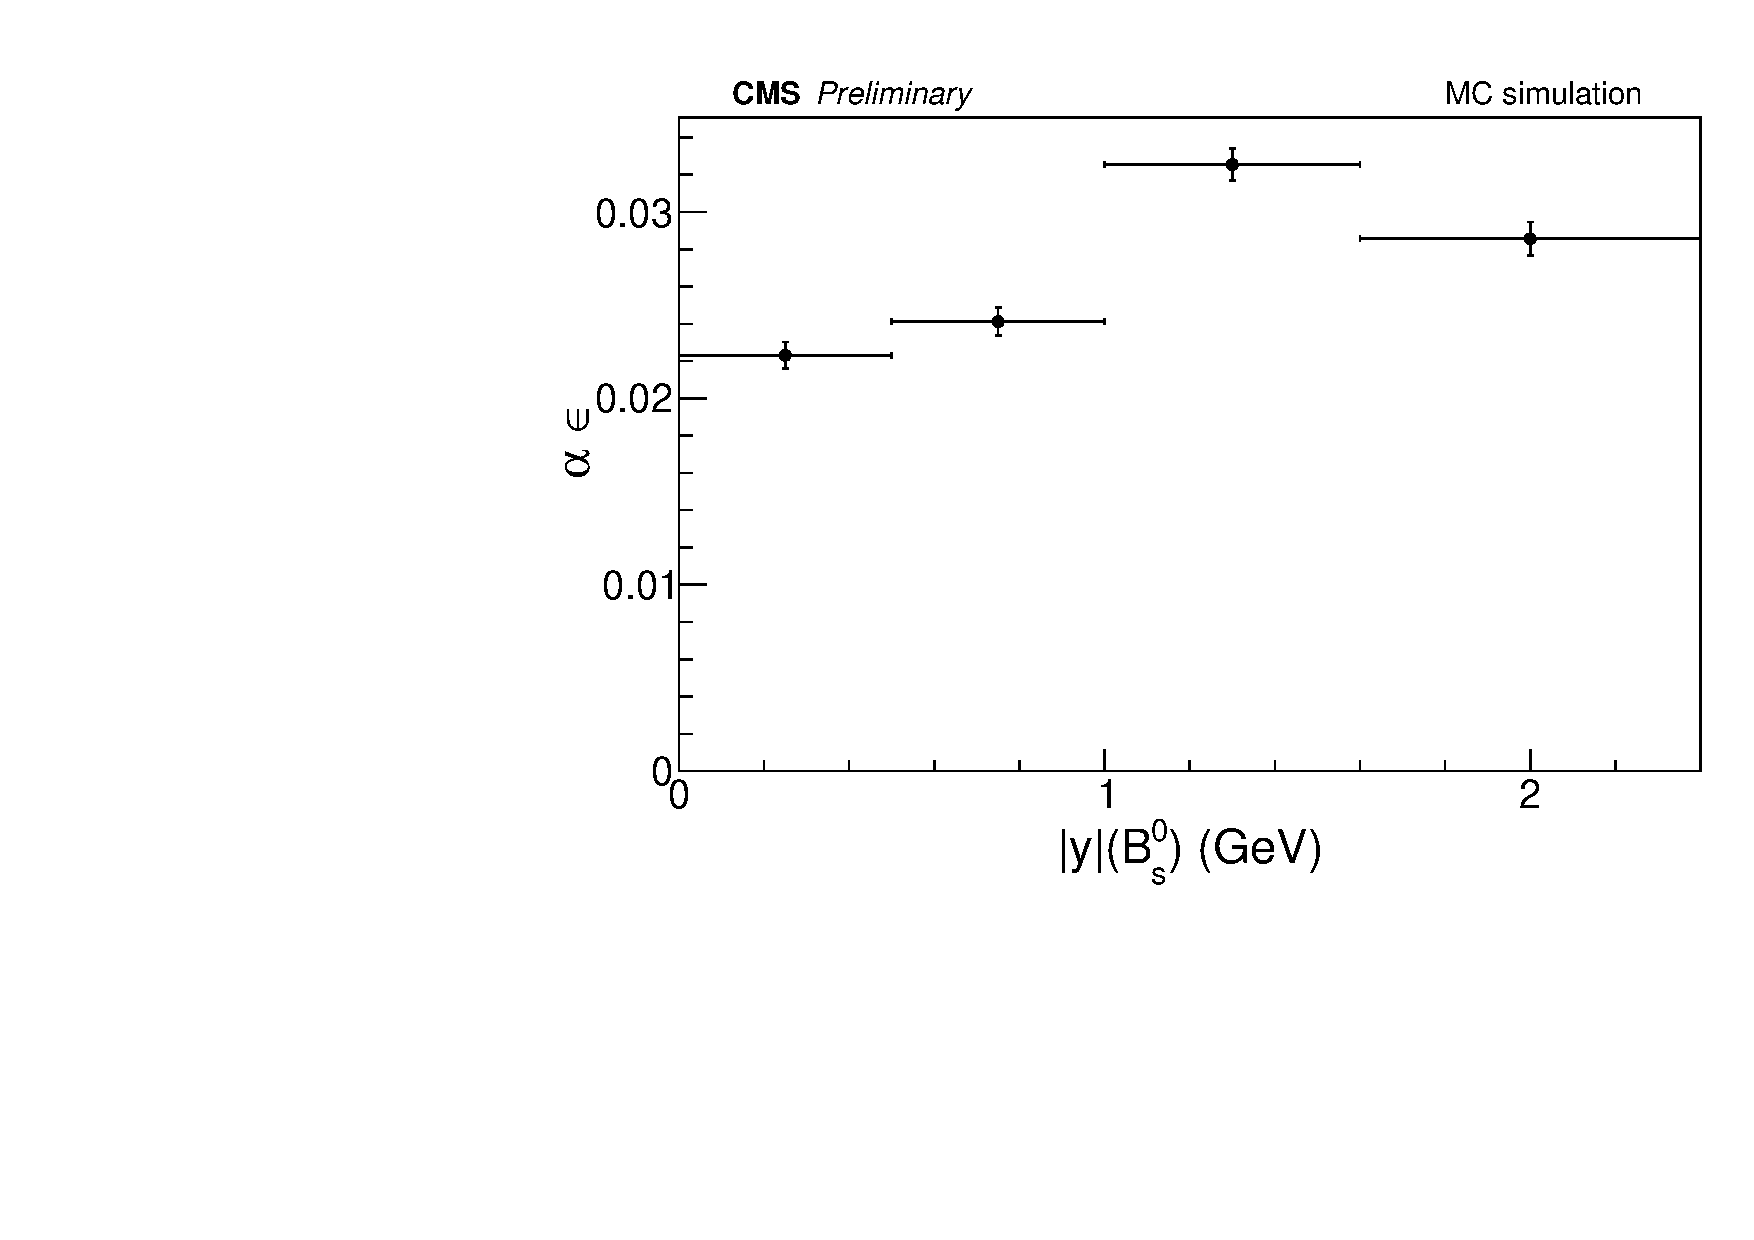
\includegraphics[width=\textwidth]{MainContent/Figs/effy/totaleffy_ybins.PDF}
		\caption{}%
	\end{subfigure}
	\caption{(a) Acceptance, (b) efficiency and (c) total efficiency for the MC simulation using $|y|$ bins.}
	\label{fig:effy_ybins}
\end{figure}

\section{Differential cross-section}

In particle physics, the term cross-section is used to express the probability of a given event occurring \cite{thomson2013modern}. More specifically, the probability that two colliding particles would interact and generate a certain event, such as the production of a specific particle \cite{pivarski2013}. The cross-section will be used in this thesis to refer to the probability of producing a $B^0_s$ meson during p-Pb collisions that decays in the manner described in \ref{subsec:channel}.

It is sometimes desirable to investigate how the cross-section is distributed with respect to a specific kinematic quantity  \cite{thomson2013modern}. This could be valuable in gaining a better understanding of the interaction. For this, the differential cross-section might be used. The differential cross-section with respect to the transverse momentum, $p_T$, is calculated as follows \cite{abe1995measurement}: 

\begin{equation}
	\label{eq:cs}
\frac{d \sigma(B_s^0 \to J/\psi\phi)}{dp_T} = \frac{N_{B^0_s}}{2 \Delta p_T \cdot \alpha \cdot \epsilon \cdot BR \cdot \mathcal{L}}
\end{equation}

where $\Delta p_T$ is the width of the $p_T$ region, $\alpha \cdot \epsilon$ is the total efficiency, BR is the branching ratio of the total decay chain, eq. \ref{eq:br}, and $\mathcal{L} = 179.7$ nb$^{-1}$  is the total integrated luminosity. Due to the quick transitions between particle and antiparticle, indicated in \ref{sec:b0s}, both $B^0_s$ and $\bar{B^0_s}$ are formed in the collision, but only $B^0_s$ is considered, for this reason, the factor $\frac{1}{2}$ is included in the equation above. Similarly, the differential cross-section for the $|y|$ bins is defined as: 

\begin{equation}
	\label{eq:cs_y}
	\frac{d \sigma(B_s^0 \to J/\psi\phi)}{d|y|} = \frac{N_{B^0_s}}{2 \Delta |y| \cdot \alpha \cdot \epsilon \cdot BR \cdot \mathcal{L}}
\end{equation}

Table \ref{table:result_raw_fdfu} shows the number of signal events, the total reconstruction efficiency and the value for the differential cross-section for the different $p_T$ bins. The top of Fig. \ref{fig:cs} depicts the results of the $p_T$ differential cross-section. The plot shows a comparison with the fixed-order plus next-to-leading-logarithm (FONLL) predictions \cite{FONLL}. The FONLL data has been calculated for pp collisions and the $B$ meson. A data escalation was performed by multiplying by the number of nucleons in the Pb nucleus, 208, and by the world average $B^{0}_s$ production fraction, $10.0 \%$ \cite{khachatryan2016study, pdgadmixture}. The error bars for the calculated differential cross-section represent systematic and statistical uncertainty. These will be discussed further in the following section. Table \ref{table:mc_ybins} and fig. \ref{fig:cs_y} show the results for the $|y|$ bins. 

\begin{table}[htbp] \begin{center}\begin{tabular}{|c|c|c|c|}\hline\textbf{$\mathbf{p_T}$ bin (GeV)} & \textbf{$\mathbf{N_{B_s^{0}}}$} & \textbf{$\mathbf{B_s^{0}}$ Total Efficiency} & \textbf{${\mathbf{\frac{d \sigma}{dp_T}}}$ ($\mu$b/GeV)} \\\hline{[}7, 10{)} &  56  $\pm$  8 &   0.0044  $\pm$  0.0002 &   375.37  $\pm$  55.77 \\{)}10, 15{)} &  116  $\pm$  12 &   0.0300  $\pm$  0.0008 &   68.17  $\pm$  6.93 \\{[}15, 20{)} &  89  $\pm$  10 &   0.0929  $\pm$  0.0026 &   16.74  $\pm$  1.92 \\{[}20, 50{)} &  104  $\pm$  11 &   0.1826  $\pm$  0.0049 &   1.67  $\pm$  0.18 \\\hline\end{tabular}\caption{The $N_{B_s^{0}}$ values obtained and efficiencies computed are shown with their respective statistical uncertainties. The value of ${\frac{d \sigma}{dp_T}}$ computed directly from these results is also shown. For ${\frac{d \sigma}{dp_T}}$, just the $N_{B_s^{0}}$ error propagation is present.}\label{table:result_raw_fdfu}\end{center}\end{table}

\begin{table}[htbp] \begin{center}\begin{tabular}{|c|c|c|c|}\hline\textbf{$\mathbf{|y|}$ bin (GeV)} & \textbf{$\mathbf{N_{B_s^{0}}}$} & \textbf{$\mathbf{B_s^{0}}$ Total Efficiency} & \textbf{${\mathbf{\frac{d \sigma}{d|y|}}}$ ($\mu$b/GeV)} \\\hline{[}0.0, 0.5{)} &  71  $\pm$  9 &   0.0223  $\pm$  0.0007 &   556.21  $\pm$  68.54 \\{[}0.5, 1.0{)} &  72  $\pm$  9 &   0.0241  $\pm$  0.0007 &   522.83  $\pm$  65.87 \\{)}1.0, 1.6{)} &  126  $\pm$  12 &   0.0325  $\pm$  0.0008 &   568.55  $\pm$  54.33 \\{[}1.6, 2.4{)} &  100  $\pm$  12 &   0.0286  $\pm$  0.0009 &   385.95  $\pm$  45.13 \\\hline\end{tabular}\caption{The $N_{B_s^{0}}$ values obtained and efficiencies computed are shown with their respective statistical uncertainties. The value of ${\frac{d \sigma}{d|y|}}$ computed directly from these results is also shown. For ${\frac{d \sigma}{d|y|}}$, just the $N_{B_s^{0}}$ error propagation is present.}\label{table:result_raw_fdfu_y}\end{center}\end{table}


It is observed that the in the center region of $p_T$, $[10, 20)$ GeV, the experimental data is closer to the FONLL prediction than in the regions of lower $p_T$, $[7, 10)$ GeV and higher $p_T$, $[20, 50)$ GeV. Nevertheless, when the double of the uncertainty for both FONLL and the experimental data is taken into account, the values fall into the $95\%$ \cite{vsirca2016probability} confidence interval. The FONLL prediction for a wider range of values is shown in the bottom of Fig. \ref{fig:cs}. The data is fitted with a curve. The total $p_T$ differential cross-section is estimated as $\frac{d \sigma}{dp_T} = (24.834 \pm 1.435(stat) \pm 5.680(sys)) \ \mu\text{b}/\text{GeV}$.

On the other hand, when considering the rapidity $|y|$, the values from FONLL and the experimental results agree when considering the total uncertainty. The value of the total $|y|$ differential cross-section is 
$\frac{d \sigma}{d|y|} = (507.34 \pm 29.31(stat) \pm 115.54(sys)) \ \mu\text{b}/\text{GeV}$.
\begin{figure*}
	\centering
	\begin{subfigure}[b]{0.7\textwidth}
		\centering
		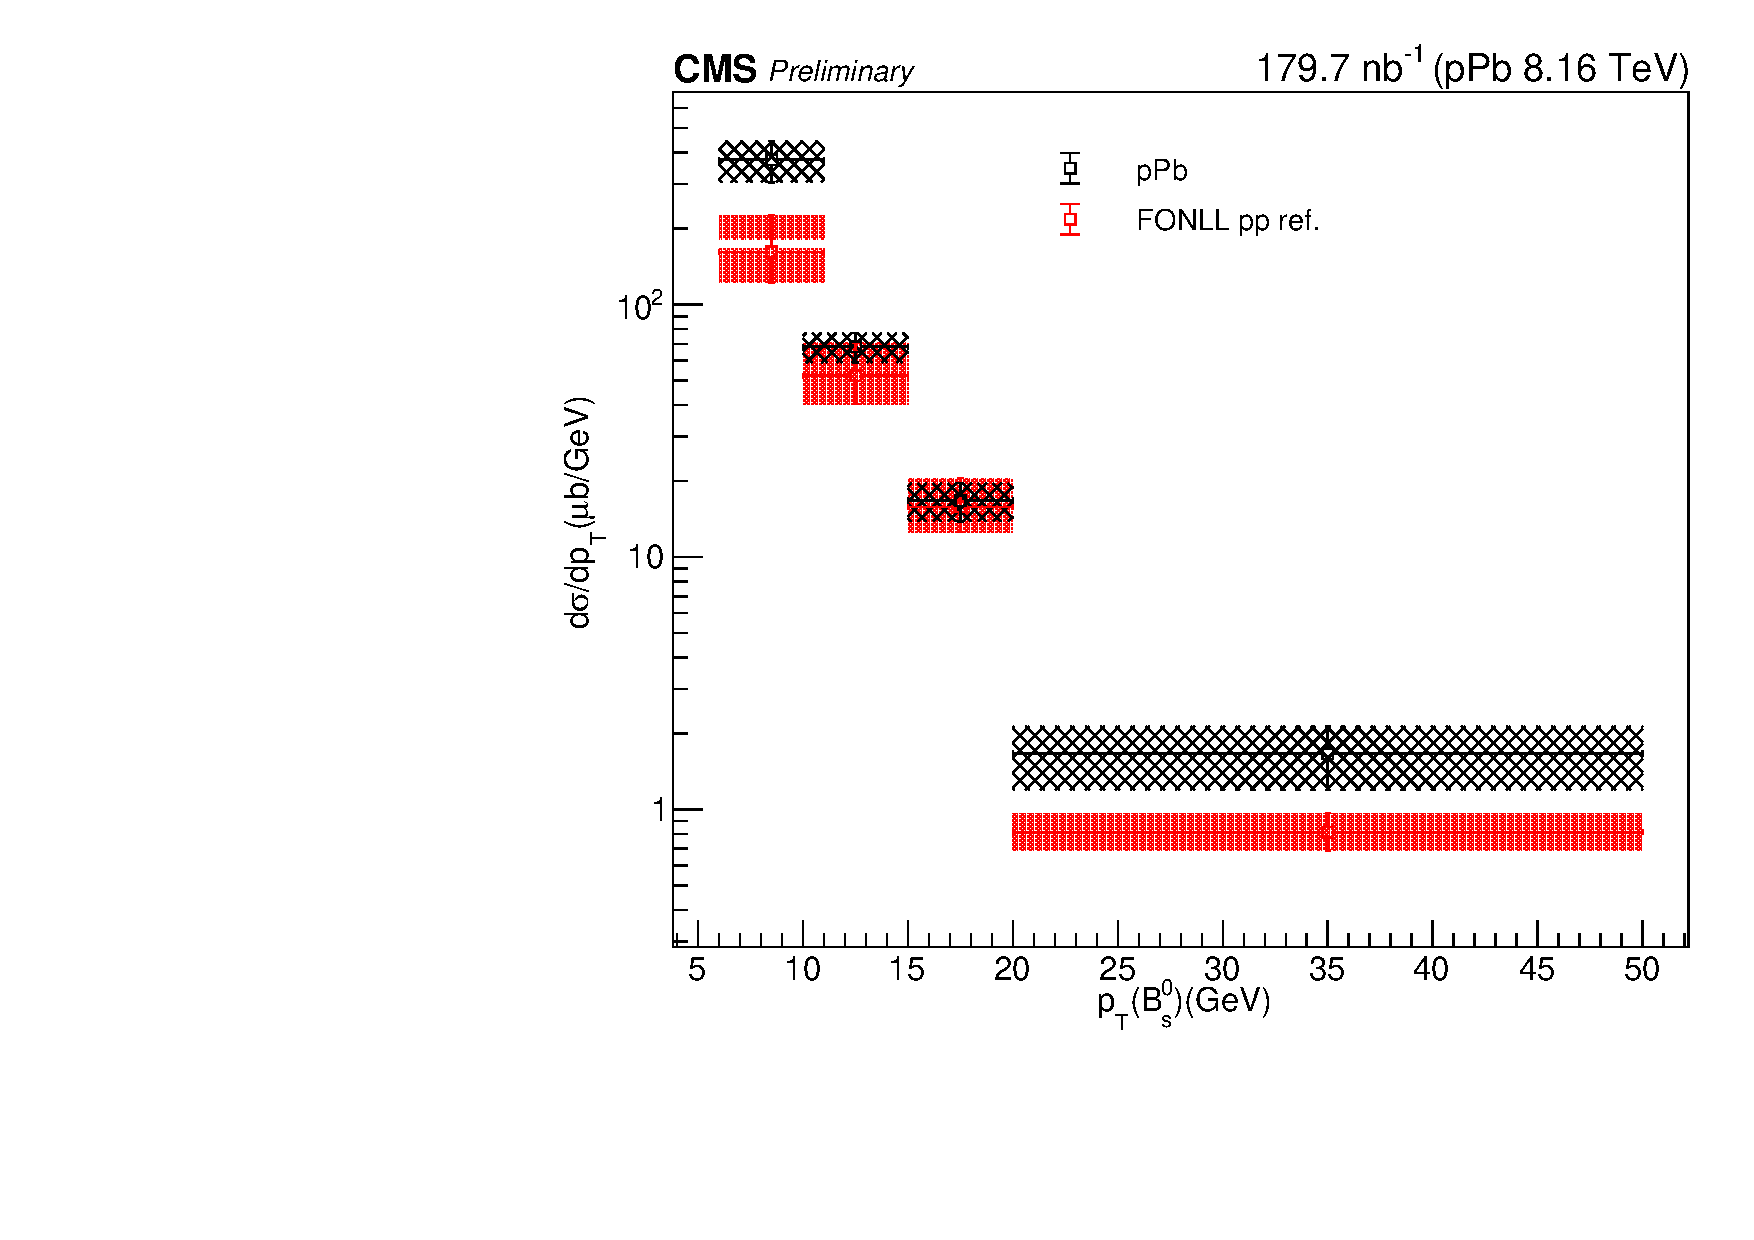
\includegraphics[width=\textwidth]{MainContent/Figs/effy/Histo_Bs_CS_pt_FONLL_8Tev.PDF}
		\caption{}%
	\end{subfigure}
	\vskip\baselineskip
	\begin{subfigure}[b]{0.7\textwidth}
		\centering
		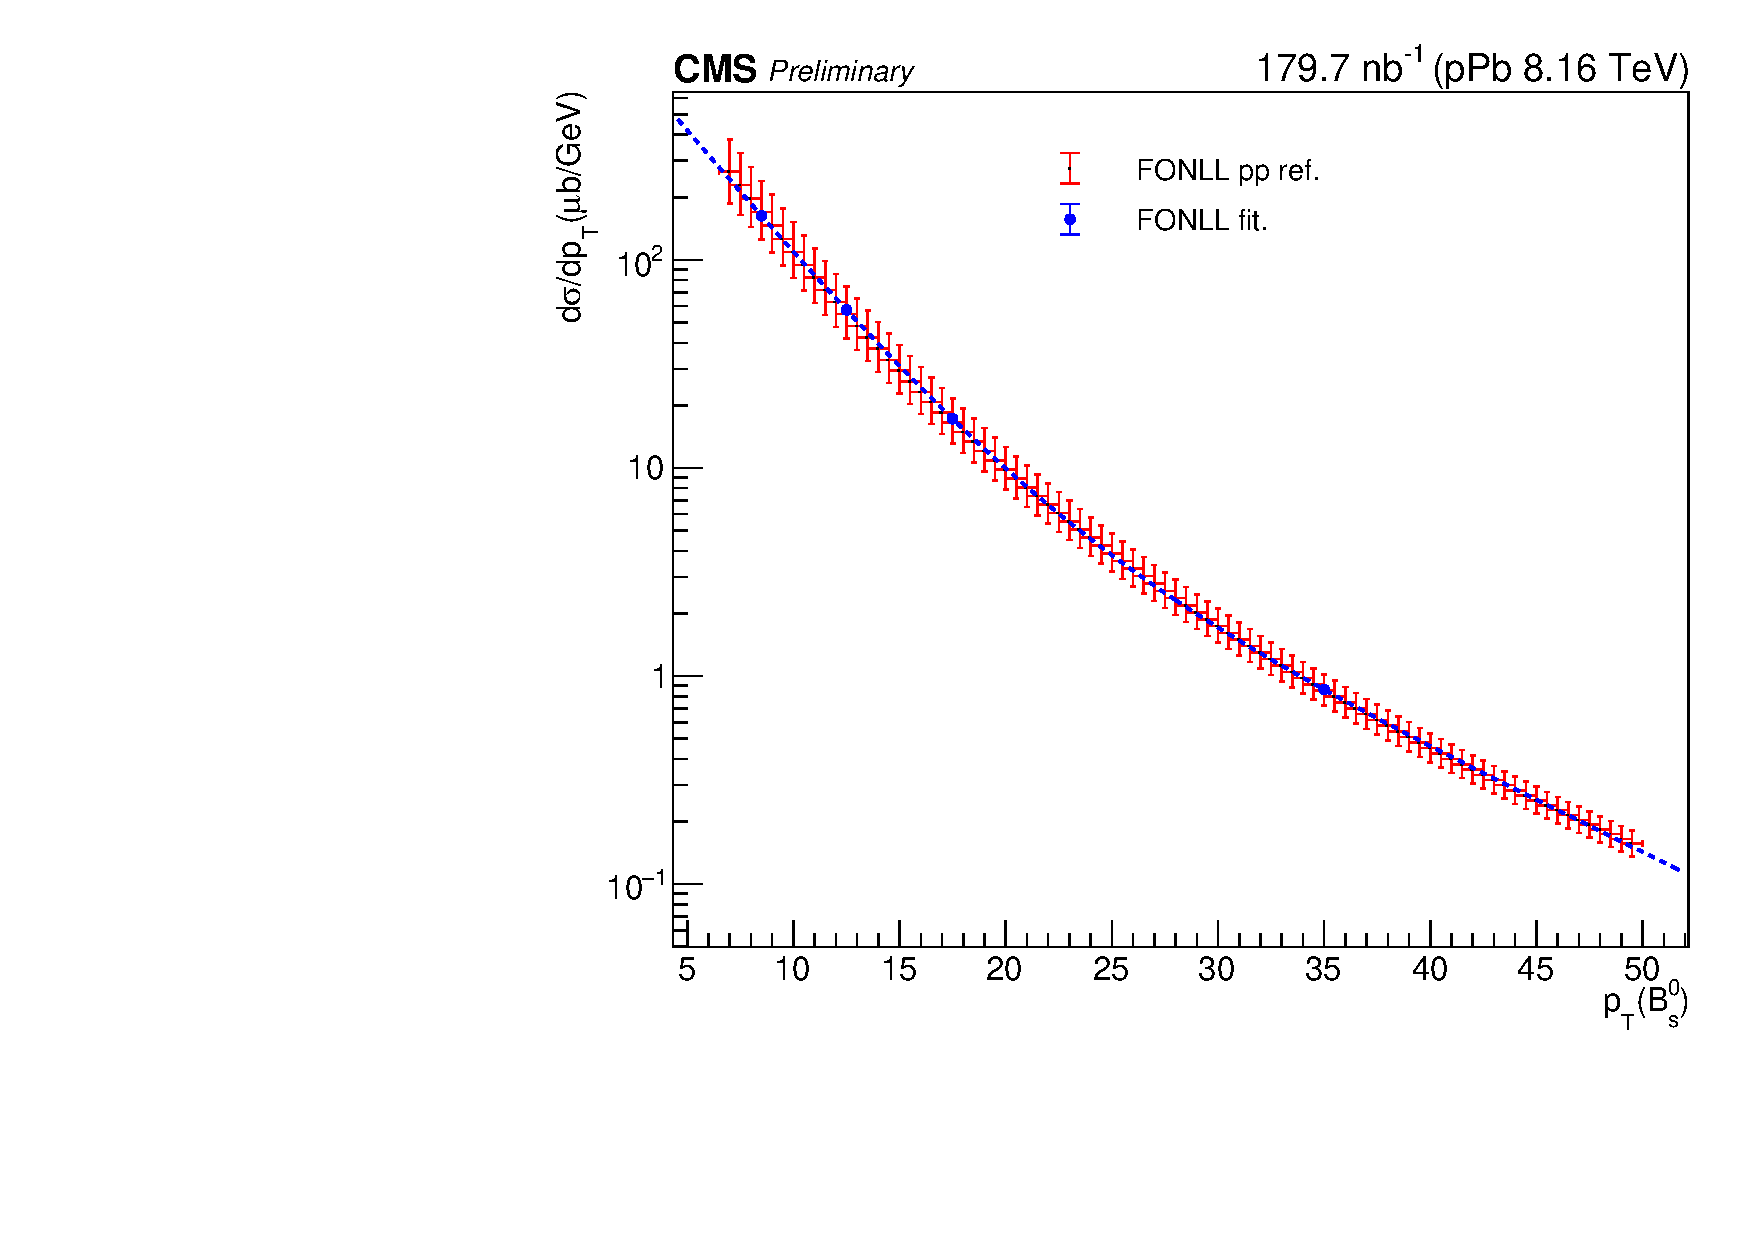
\includegraphics[width=\textwidth]{MainContent/Figs/effy/Histo_Bs_CS_pt_FONLL_8Tev_curve.PDF}
		\caption{}%
	\end{subfigure}
	\caption{$p_T$ Differential cross-section for the $B^0_s$ meson, where a) corresponds to a comparison between predicted and calculated values and b) full plot of predicted values.}
	\label{fig:cs}
\end{figure*}

\begin{figure*}
	\centering
	\begin{subfigure}[b]{0.7\textwidth}
		\centering
		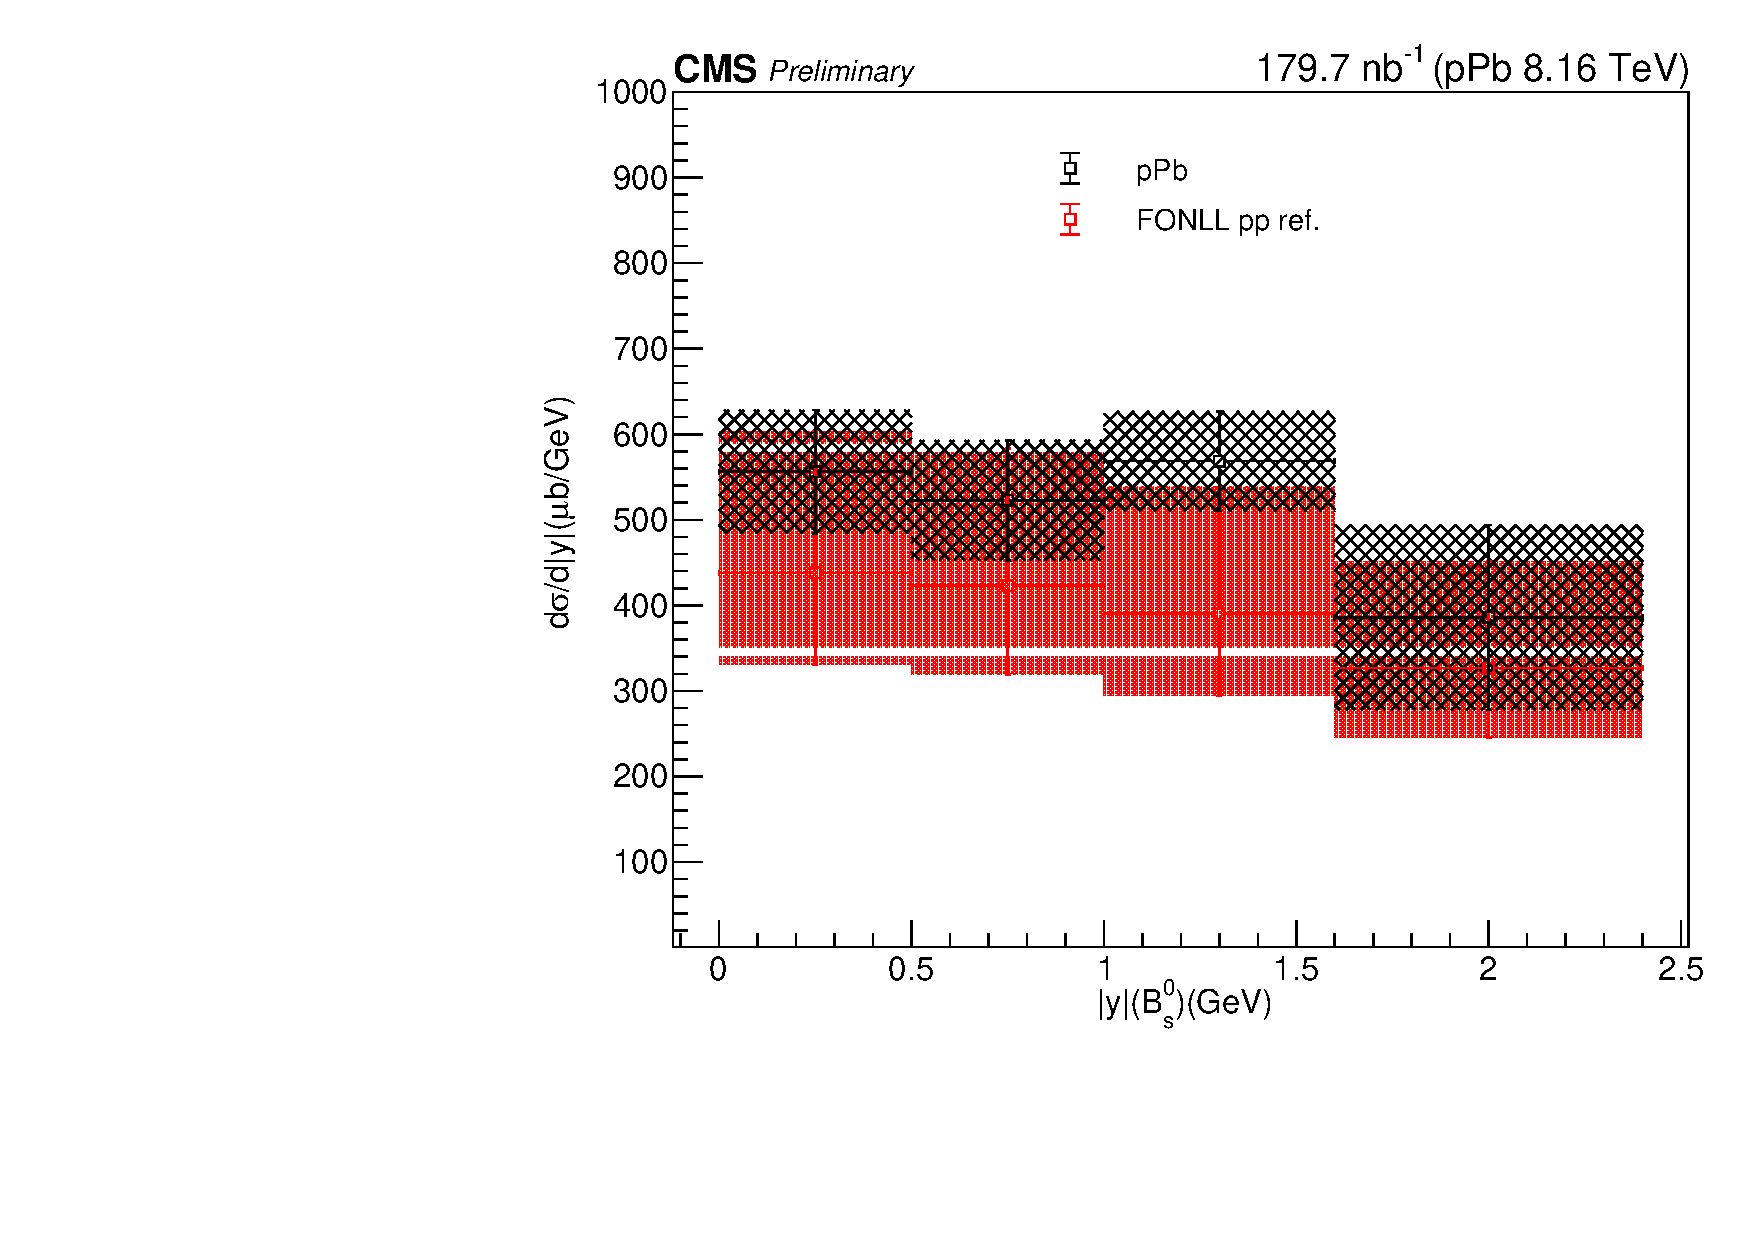
\includegraphics[width=\textwidth]{MainContent/Figs/effy/Histo_Bs_CS_y_FONLL_8Tev.PDF}
		\caption{}%
	\end{subfigure}
	\vskip\baselineskip
	\begin{subfigure}[b]{0.7\textwidth}
		\centering
		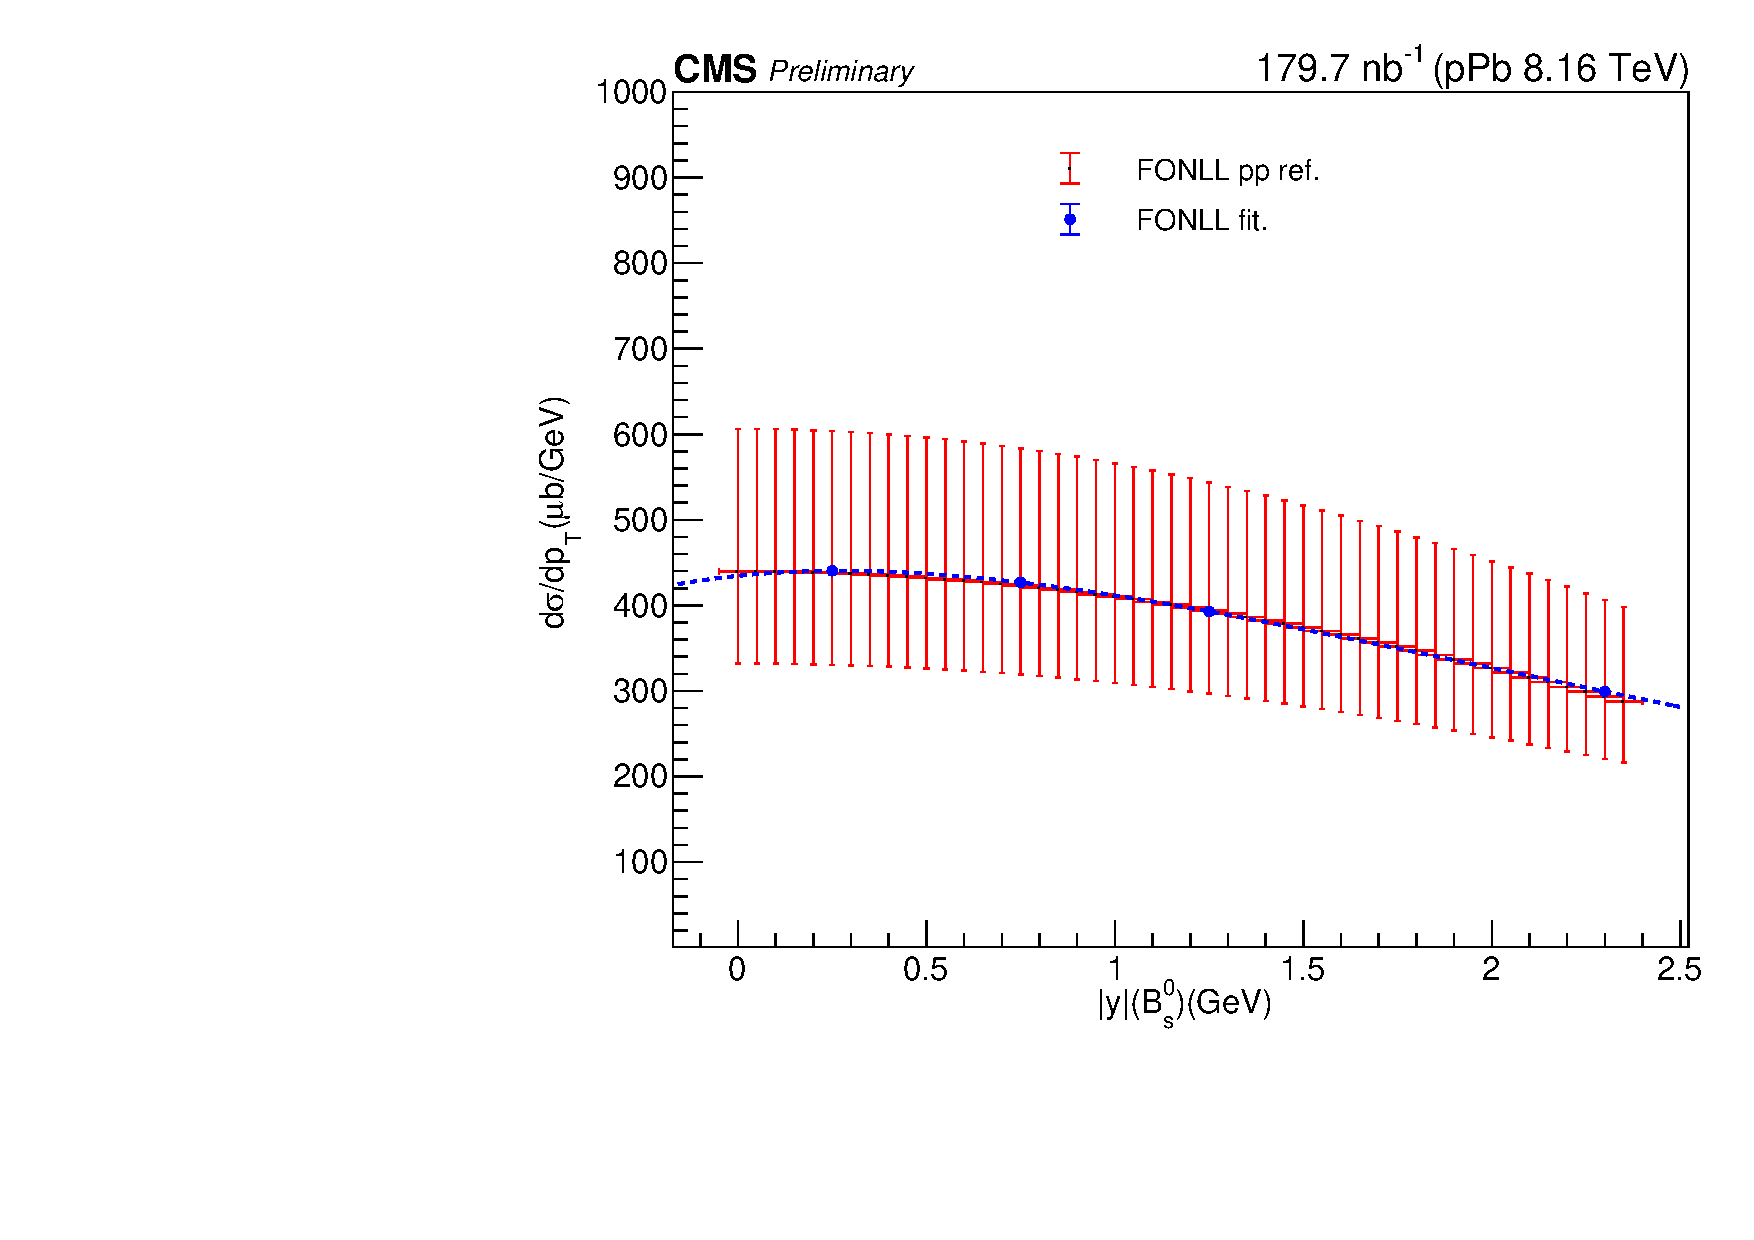
\includegraphics[width=\textwidth]{MainContent/Figs/effy/Histo_Bs_CS_y_FONLL_8Tev_curve_ybins.PDF}
		\caption{}%
	\end{subfigure}
	\caption{$|y|$ differential cross-section for the $B^0_s$ meson, where a) corresponds to a comparison between predicted and calculated values and b) full plot of predicted values.}
	\label{fig:cs_y}
\end{figure*}

 \cleardoublepage
\section{Uncertainty in the differential cross-section}
The uncertainties in the measurement of a quantity during a physics experiment can be classified by two types. The first type are the statistical uncertainties, which are related to the fact that multiple measurements of the same quantity can yield different results. Therefore, the value of such quantity is not precise, but fluctuates within a range. The measurement of this range is the statistical uncertainty \cite{sinervo2003definition}. The statistical uncertainties are calculated by \verb|ROOTFIT|, and in the case of the ML method, these are determined by the covariance matrix $\mathrm{var}[\vec{\Theta}]$ \cite{vsirca2016probability}:

\begin{equation}
	\mathrm{var}[\vec{\Theta}] = 
	\left(-E\left[ \frac{\partial^2 l(x | \vec{\Theta}) }{\partial \vec{\Theta} ^2}\right]_{\Theta = \hat{\Theta}}\right)^{-1}
\end{equation}

with $E[X]$ the expected value of $X$. The diagonals are the variance of the parameters $\vec{\Theta}$ and the uncertainty is the square root of the variance, 

\begin{equation}
	\delta \Theta_i = \sqrt{\mathrm{var}[\Theta_i]}
\end{equation}

On the other hand, given a set of $N$ random variables $\vec{X}$ and a respective covariance matrix $\mathrm{var}[\vec{X}]$, if a function $f = f(\vec{X})$ depends on these variables, then the variance associated to $f$ is calculated by \cite{vsirca2016probability}:

\begin{equation}
	\mathrm{var}[f(\vec{X})] = \sum_{i=1}^N \sum_{j=1}^N \left(\frac{\partial f}{\partial X_i} \frac{\partial f}{\partial X_j} \right)_{X = \mu} \mathrm{var}[\vec{X}]_{i,j}
\end{equation}

with the partial derivatives evaluated at the mean value of $X$, $\mu$. When there is no correlation between variables, the previous equation reduces to:

\begin{equation}
	\label{totaluncertainty}
	\mathrm{var}[f(\vec{X})] = \sum_{i=1}^N  \left(\frac{\partial f}{\partial X_i}\right)^2_{X = \mu} \mathrm{var}[X_i]
\end{equation}

Revise \cite{vsirca2016probability} for more information on expected values, variance, and their relation to uncertainties. Alternatively, any statistical book on the subject would suffice.

The second type are systematic uncertainties. They are related to the nature of the instrument used, the specific model chosen for the data, the assumptions made about the experiment beforehand, among other factors. It should be noted that by taking more measurements of the quantity, the value of the statistical uncertainty can be minimized. For systematic uncertainties, however, this is not the case \cite{sinervo2003definition}. The uncertainties from different measurements are correlated, which means that they are not independent of one another. After a thorough examination and testing of the potential sources of uncertainty, systematic uncertainties can be calculated and possibly reduced. The total systematic uncertainty is calculated as:

\begin{equation}
	\delta_{sys} = \sqrt{\sum_{i}^{N} \delta_{{sys}_{i}}^2}
\end{equation}

where $\delta_{{sys}_i}$ represents each one of the individual systematic uncertainties.
%\begin{equation}
%	\delta_T = \sqrt{\delta_{stat}^2 + \delta_{sys}^2}
%\end{equation}

In the estimation of the uncertainty of the differential cross-section, several sources of statistical and systematic uncertainties are to be considered. By using eq. \ref{totaluncertainty} in eq. \ref{eq:cs} and eq. \ref{eq:cs_y}, the total statistical uncertainty can be obtained:

\begin{equation}
	\delta \left(\frac{d\sigma(B_s^0)}{dp_T} \right)_{stat} 
 =\frac{d \sigma(B_s^0)}{dp_T}\left| \frac{\delta N_{B_s^{0}}}{N_{B_s^{0}}}\right|
 \end{equation}

\begin{equation}
	\delta \left(\frac{d\sigma(B_s^0)}{d|y|} \right)_{stat} 
	=\frac{d \sigma(B_s^0)}{d|y|}\left| \frac{\delta N_{B_s^{0}}}{N_{B_s^{0}}}\right|
\end{equation}

In this situation, only the number of signal events $N_{B_s^{0}}$ is taken into account. An explanation on how to determine the sources of systematic uncertainties is provided below. 

\subsection{Fit model}

The influence of the signal and background PDFs is analyzed independently to establish the systematic uncertainty deriving from the chosen invariant mass PDF. To accomplish this, one of the PDFs is maintained unmodified, while the other is replaced with a PDF that is also suitable for the data.

As described in section \ref{mlmethod}, the signal PDF has fixed parameters, therefore, a PDF with free parameters is used. Once the fit is completed, a second value for the number of signal events is obtained $N_{B_s^{0}}'$, and the difference between the original value and $N_{B_s^{0}}'$ is considered the source of systematic uncertainty in the signal model, $\sigma_{sig}$.

The systematic uncertainties from the background are calculated in a similar fashion. The background PDF is replaced by a PDF consisting of a linear combination of Chebyshev polynomials of the first kind:

\begin{equation}
	B_{PDF}^{'}(M_i) = \sum_{i=0}^{N} c_i T_i(M_i) 
\end{equation}

with \cite{mason2002chebyshev} $T_i(M_i) = \cos(iM_i)$ and $c_i$ the coefficients. The \verb|ROOTFIT| library assumes that for $T_0 = 1$, the coefficient is simply $c_i = 1$ \cite{chebyshev}. Using this model, the number of background events may change, leading to a different value in the number of signal events  $N_{B_s^{0}}''$, thus, a systematic uncertainty from the background model, $\sigma_{bkg}$, can be calculated from the difference between $N_{B_s^{0}}$ and $N_{B_s^{0}}''$. The results in $p_T$ bins for systematic signal model are presented in Fig. \ref{fig:mass_ptbins_syssig} and for the background model in Fig. \ref{fig:mass_ptbins_sysbkg}. The total region is considered in Fig. \ref{fig:mass_ptbins_sys} for both cases. Figs. \ref{fig:mass_ybins_syssig} and \ref{fig:mass_ybins_sysbkg} present these results for the case of the $|y|$ bins. When comparing different models for signal and background, there are minor differences in the invariant mass and $\sigma$, as well as more significant differences in the number of signal events. However, the number of background events does not change. Since there is a small number of background events, the complexity of the fit is relatively low and both models perform similarly.

\begin{figure}[htp!]
	\centering
	\centering
	\begin{subfigure}[b]{0.475\textwidth}
		\centering
		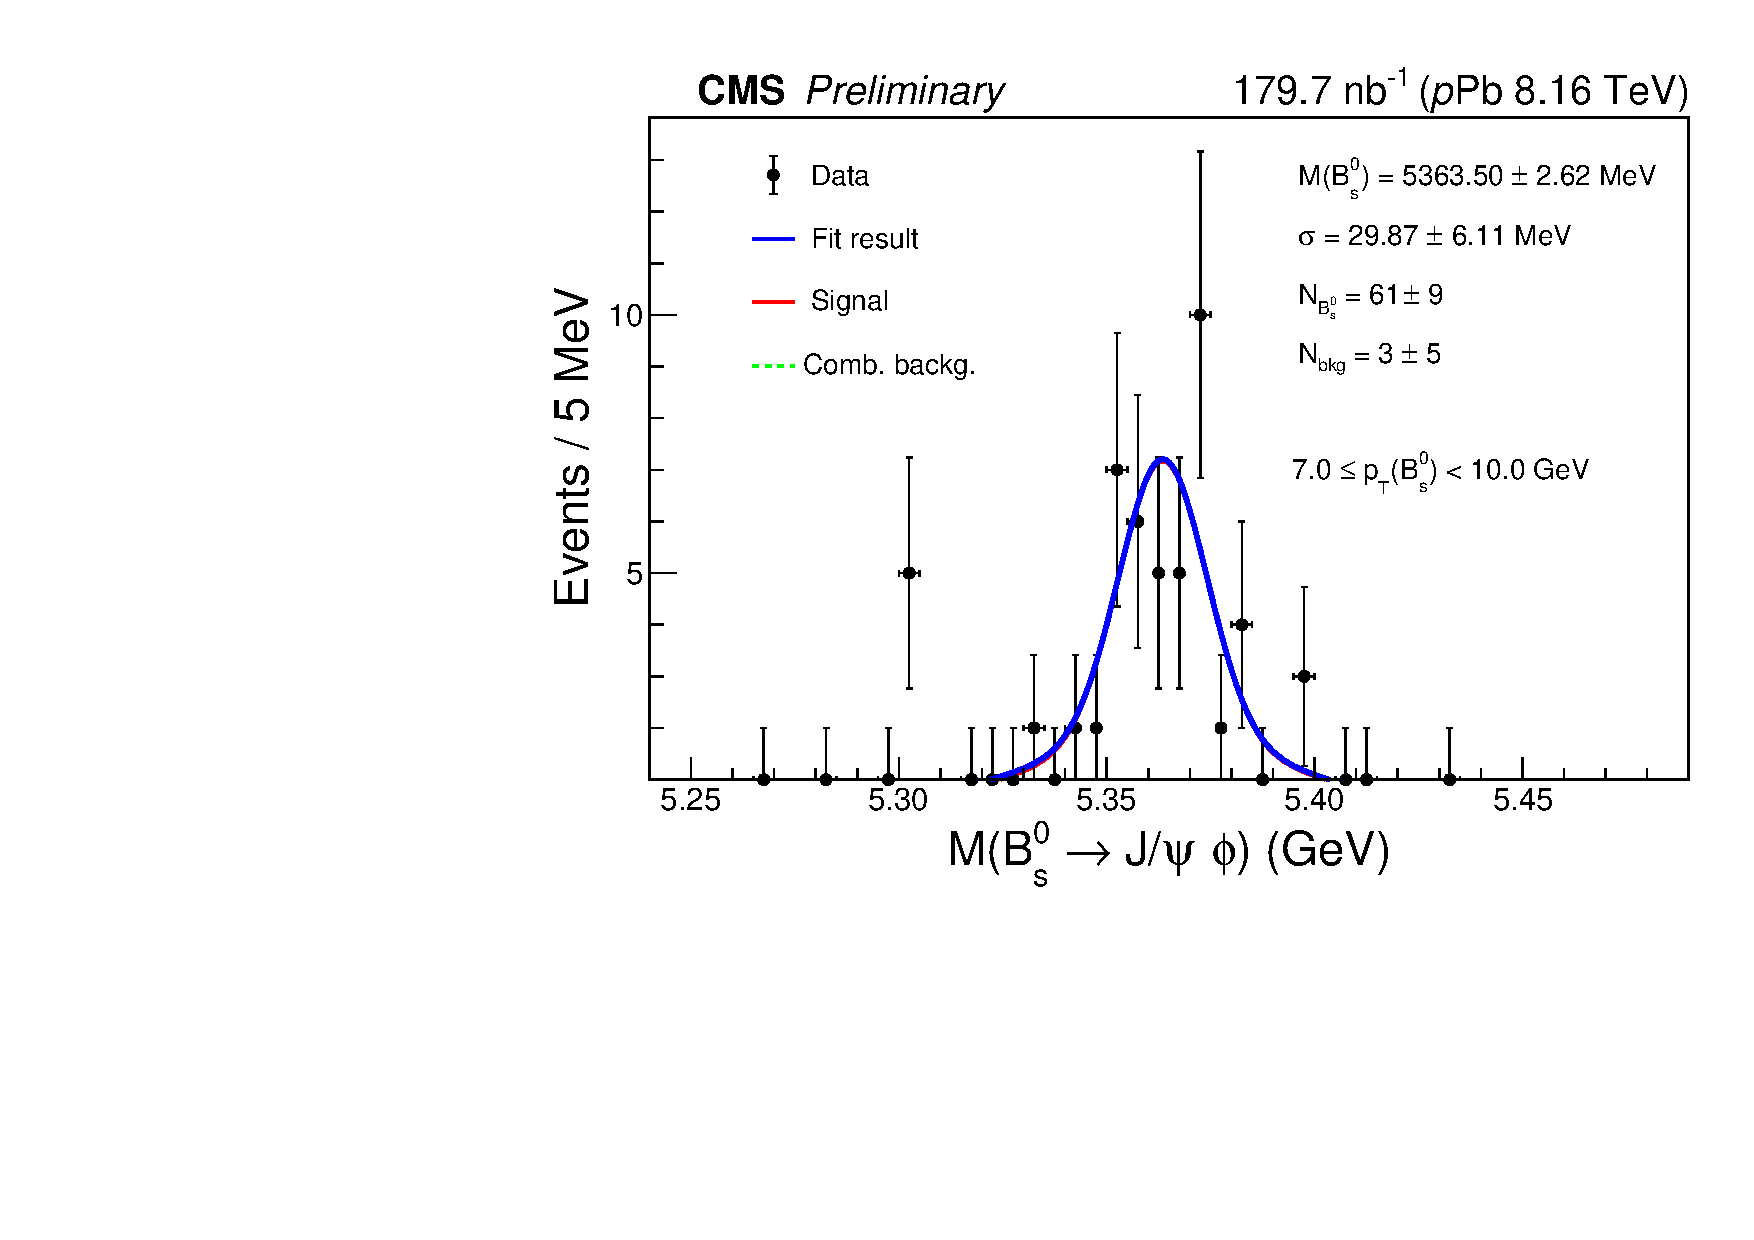
\includegraphics[width=\textwidth]{MainContent/Figs/mass/mass_BsFit_ptbins_syssig_7_10.PDF}
		\caption{}%
	\end{subfigure}
	\hfill
	\begin{subfigure}[b]{0.475\textwidth}
		\centering
		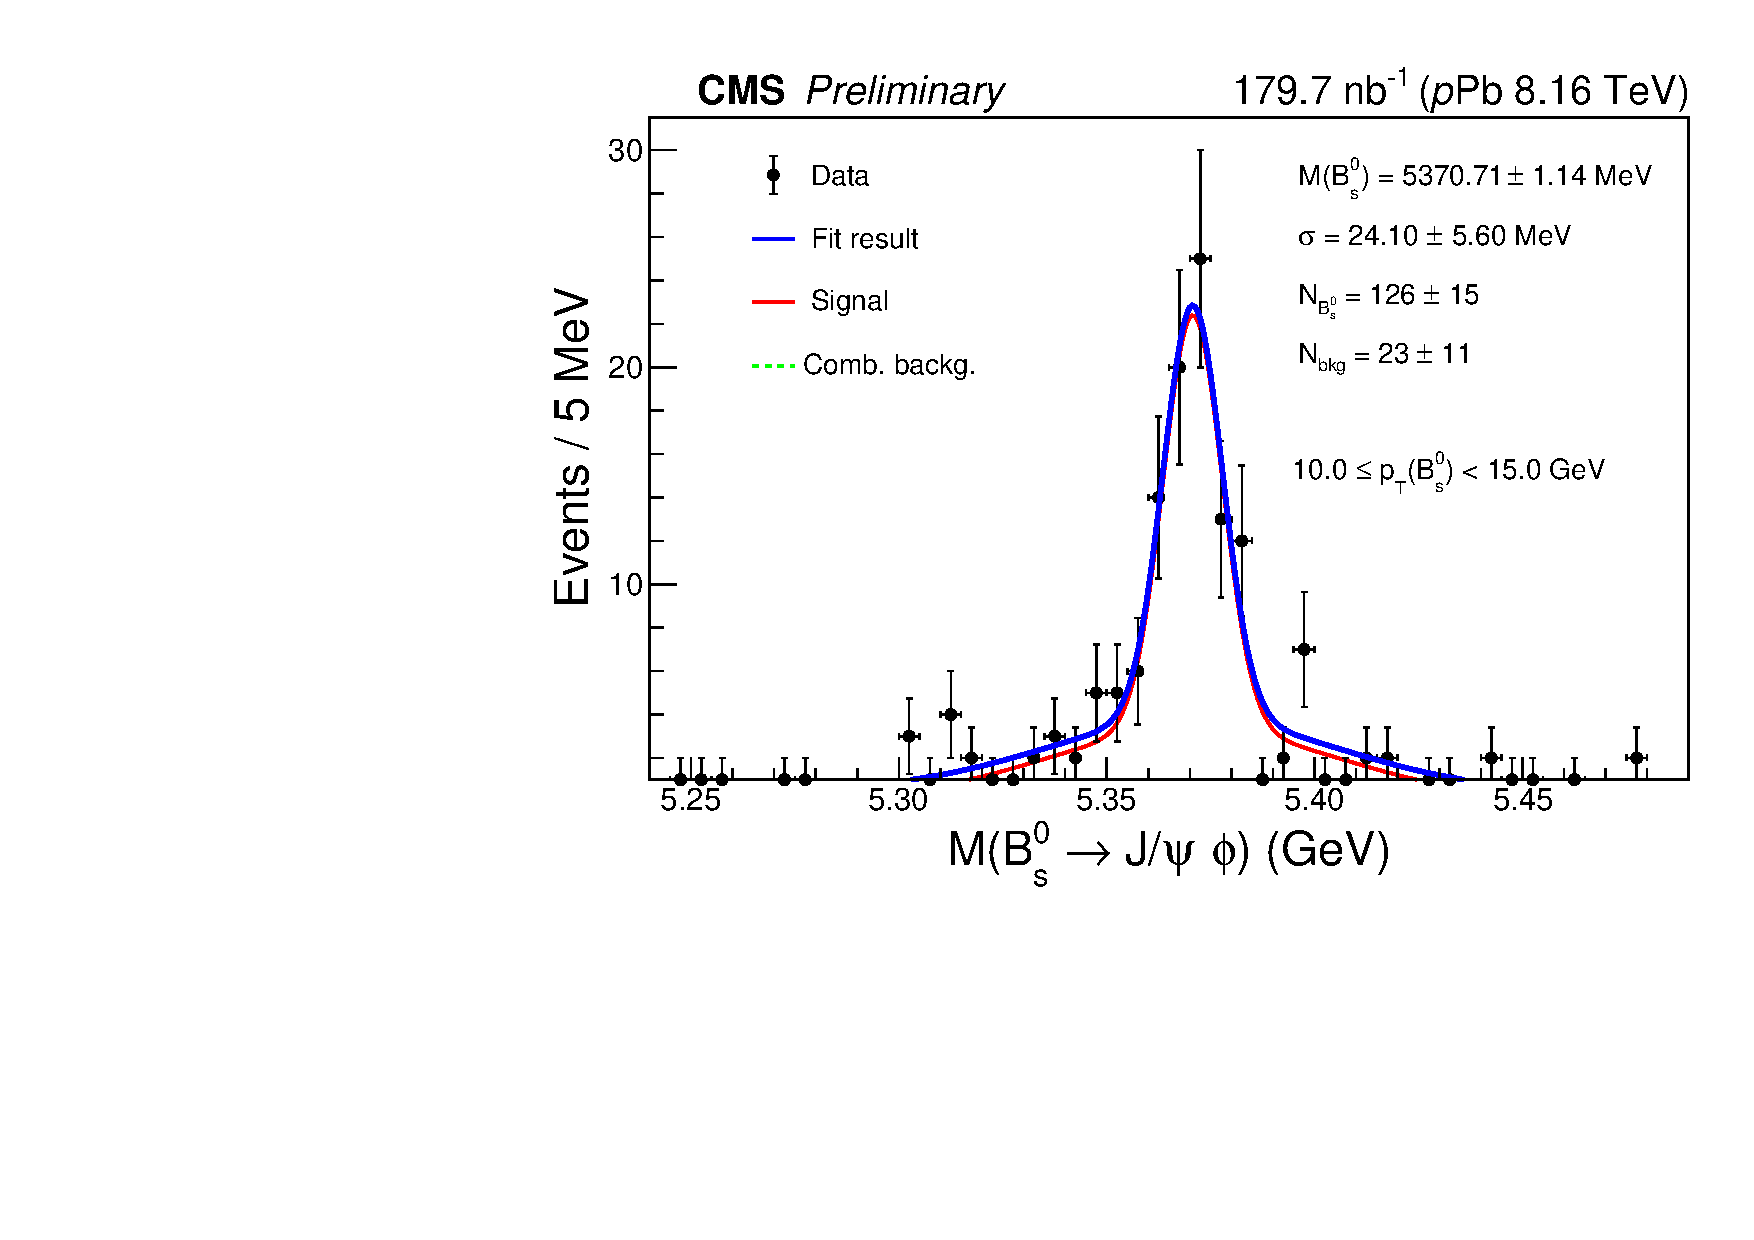
\includegraphics[width=\textwidth]{MainContent/Figs/mass/mass_BsFit_ptbins_syssig_10_15.PDF}
		\caption{}%
	\end{subfigure}
	\vskip\baselineskip
	\begin{subfigure}[b]{0.475\textwidth}
		\centering
		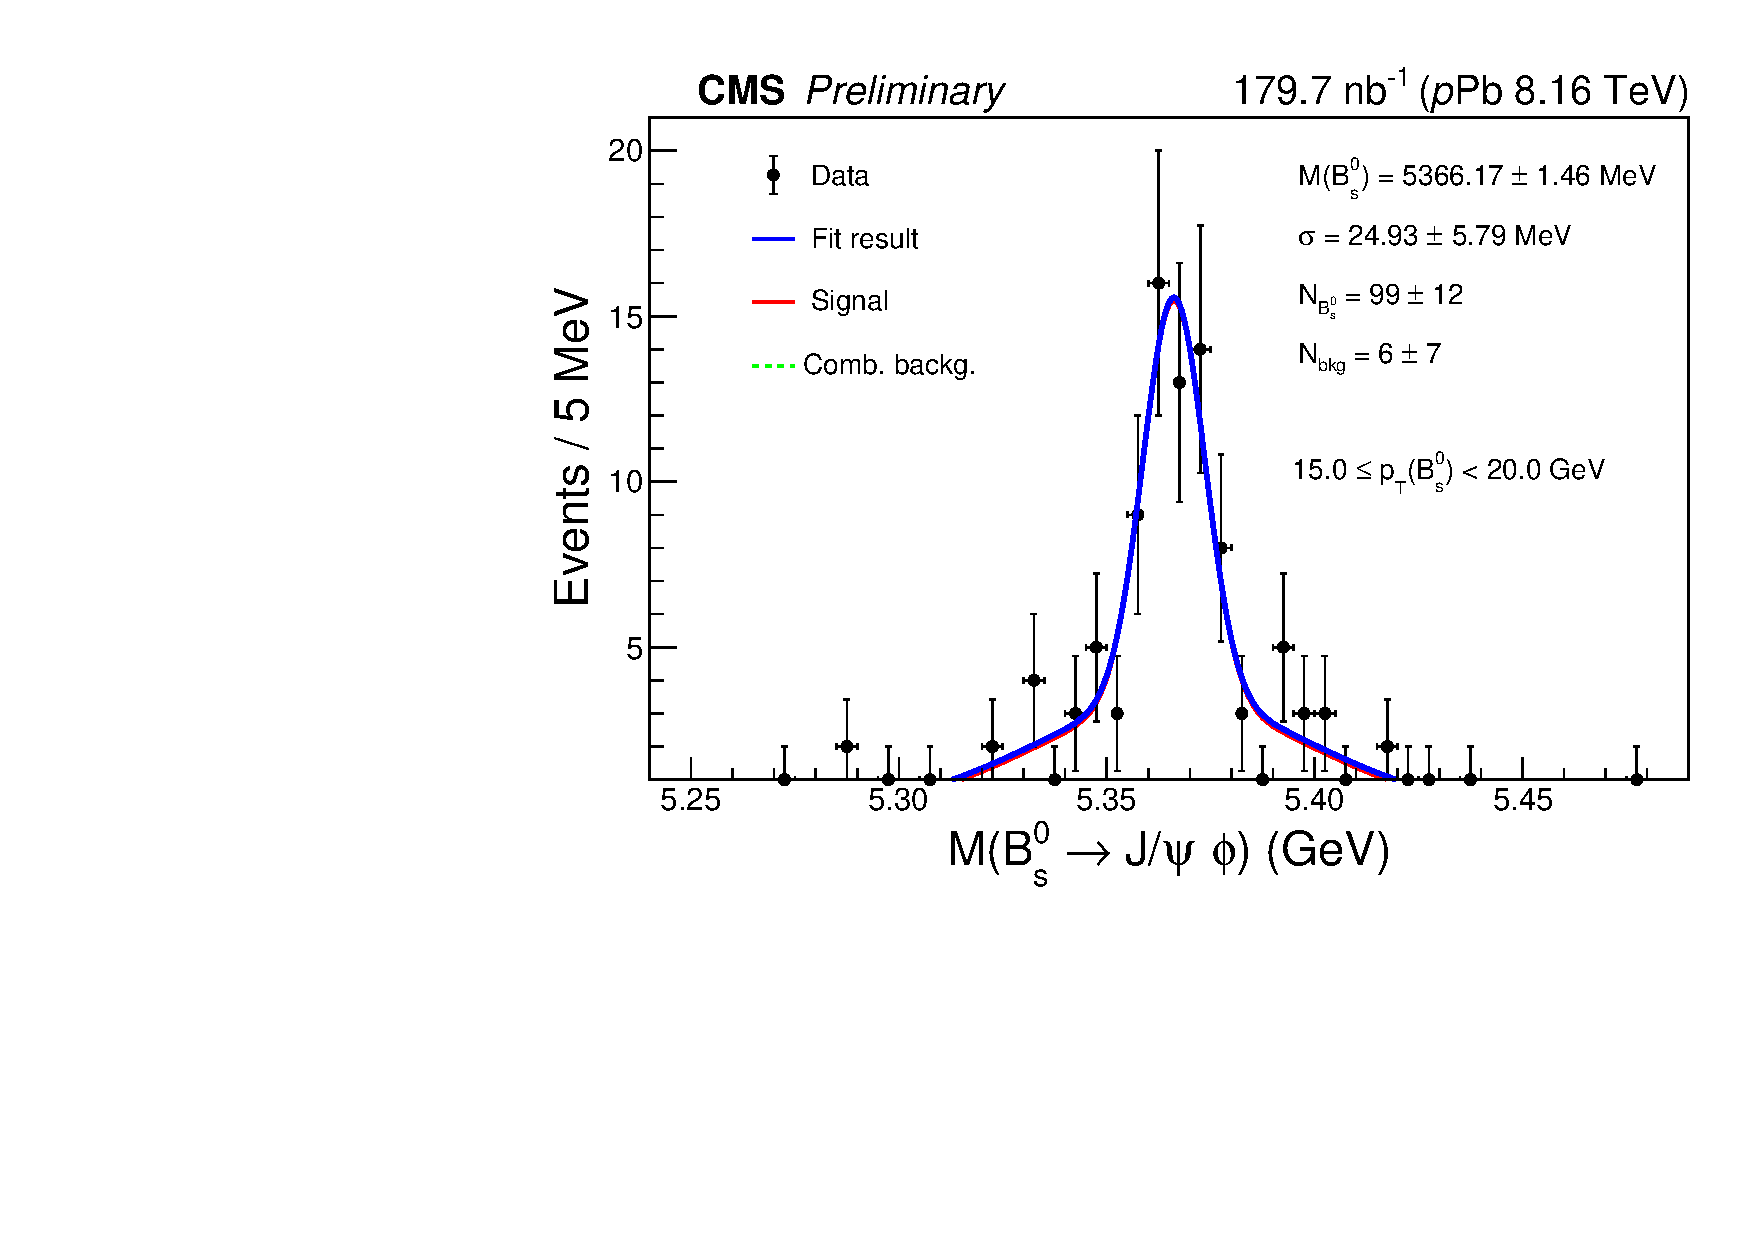
\includegraphics[width=\textwidth]{MainContent/Figs/mass/mass_BsFit_ptbins_syssig_15_20.PDF}
		\caption{}
	\end{subfigure}
	\hfill
	\begin{subfigure}[b]{0.475\textwidth}
		\centering
		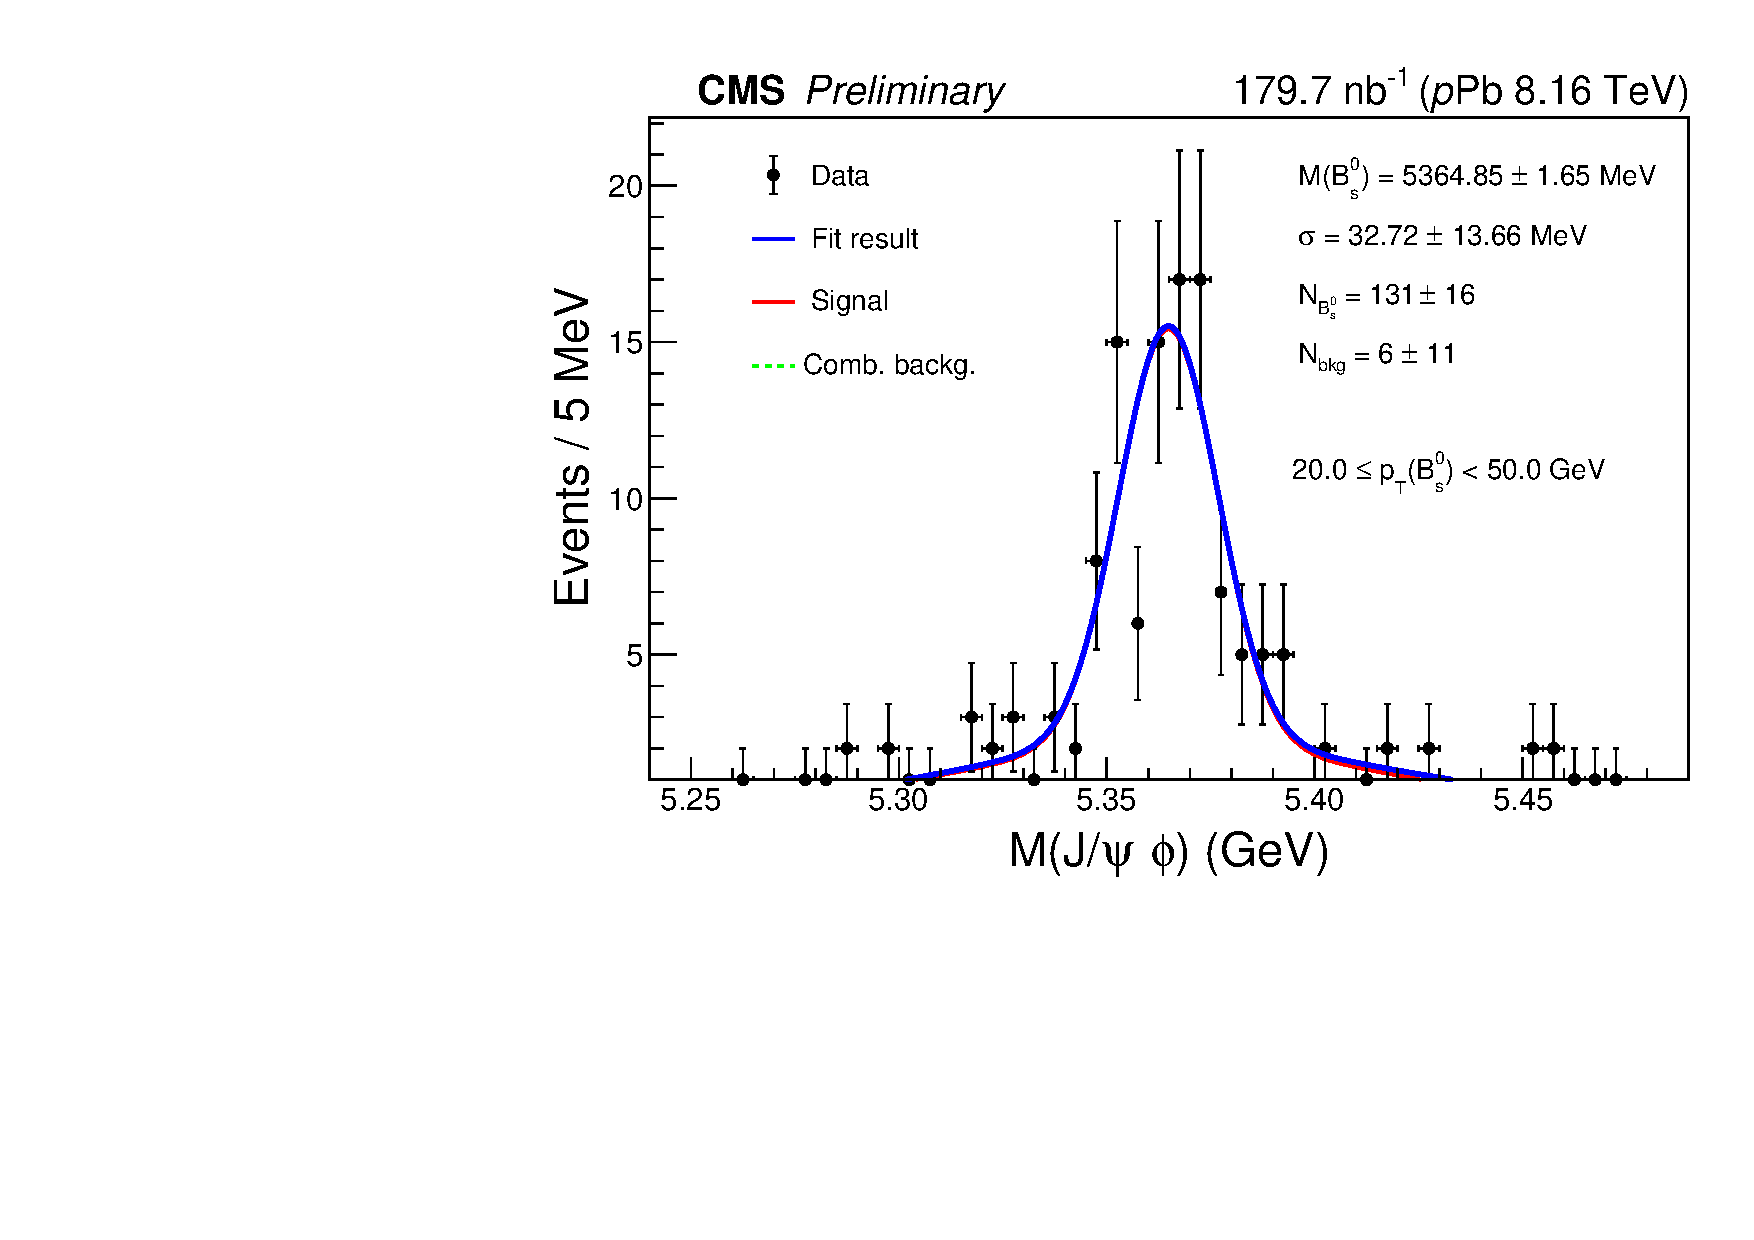
\includegraphics[width=\textwidth]{MainContent/Figs/mass/mass_BsFit_ptbins_syssig_20_50.PDF}
		\caption{}%
	\end{subfigure}
	\caption{Invariant mass spectra for $B^0_s$ meson reconstructed from the combined system $J/\psi \phi$ and considering a systematic model for signal. Four intervals for the transverse momentum $p_T(B^0_s)$ have been considered.}
	\label{fig:mass_ptbins_syssig}
	%%%%%%%%%%%%%%%%%%%%%%%%%%%%%%%%%%%%second row
	
\end{figure}

\begin{figure}[htp!]
	\centering
	\centering
	\begin{subfigure}[b]{0.475\textwidth}
		\centering
		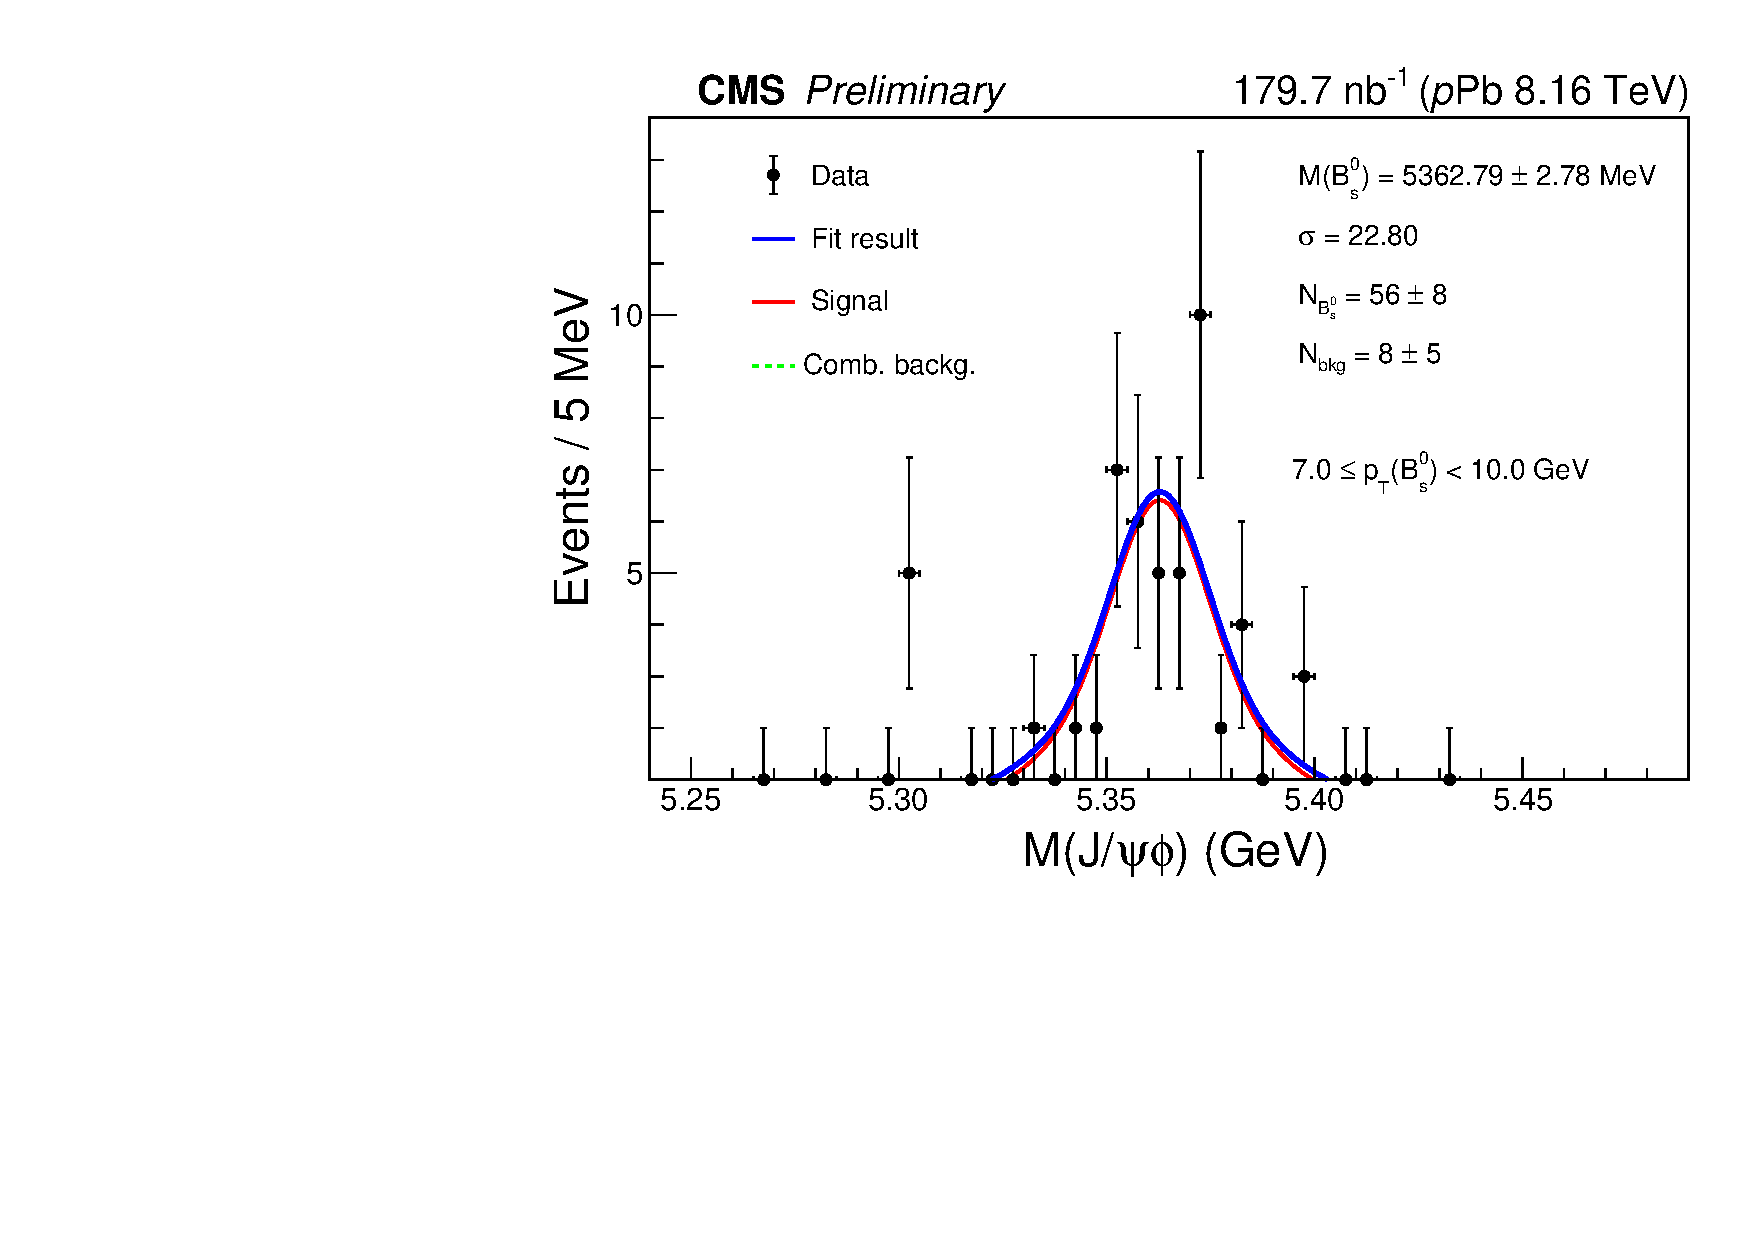
\includegraphics[width=\textwidth]{MainContent/Figs/mass/mass_BsFit_ptbins_sysbkg_7_10.PDF}
		\caption{}%
	\end{subfigure}
	\hfill
	\begin{subfigure}[b]{0.475\textwidth}
		\centering
		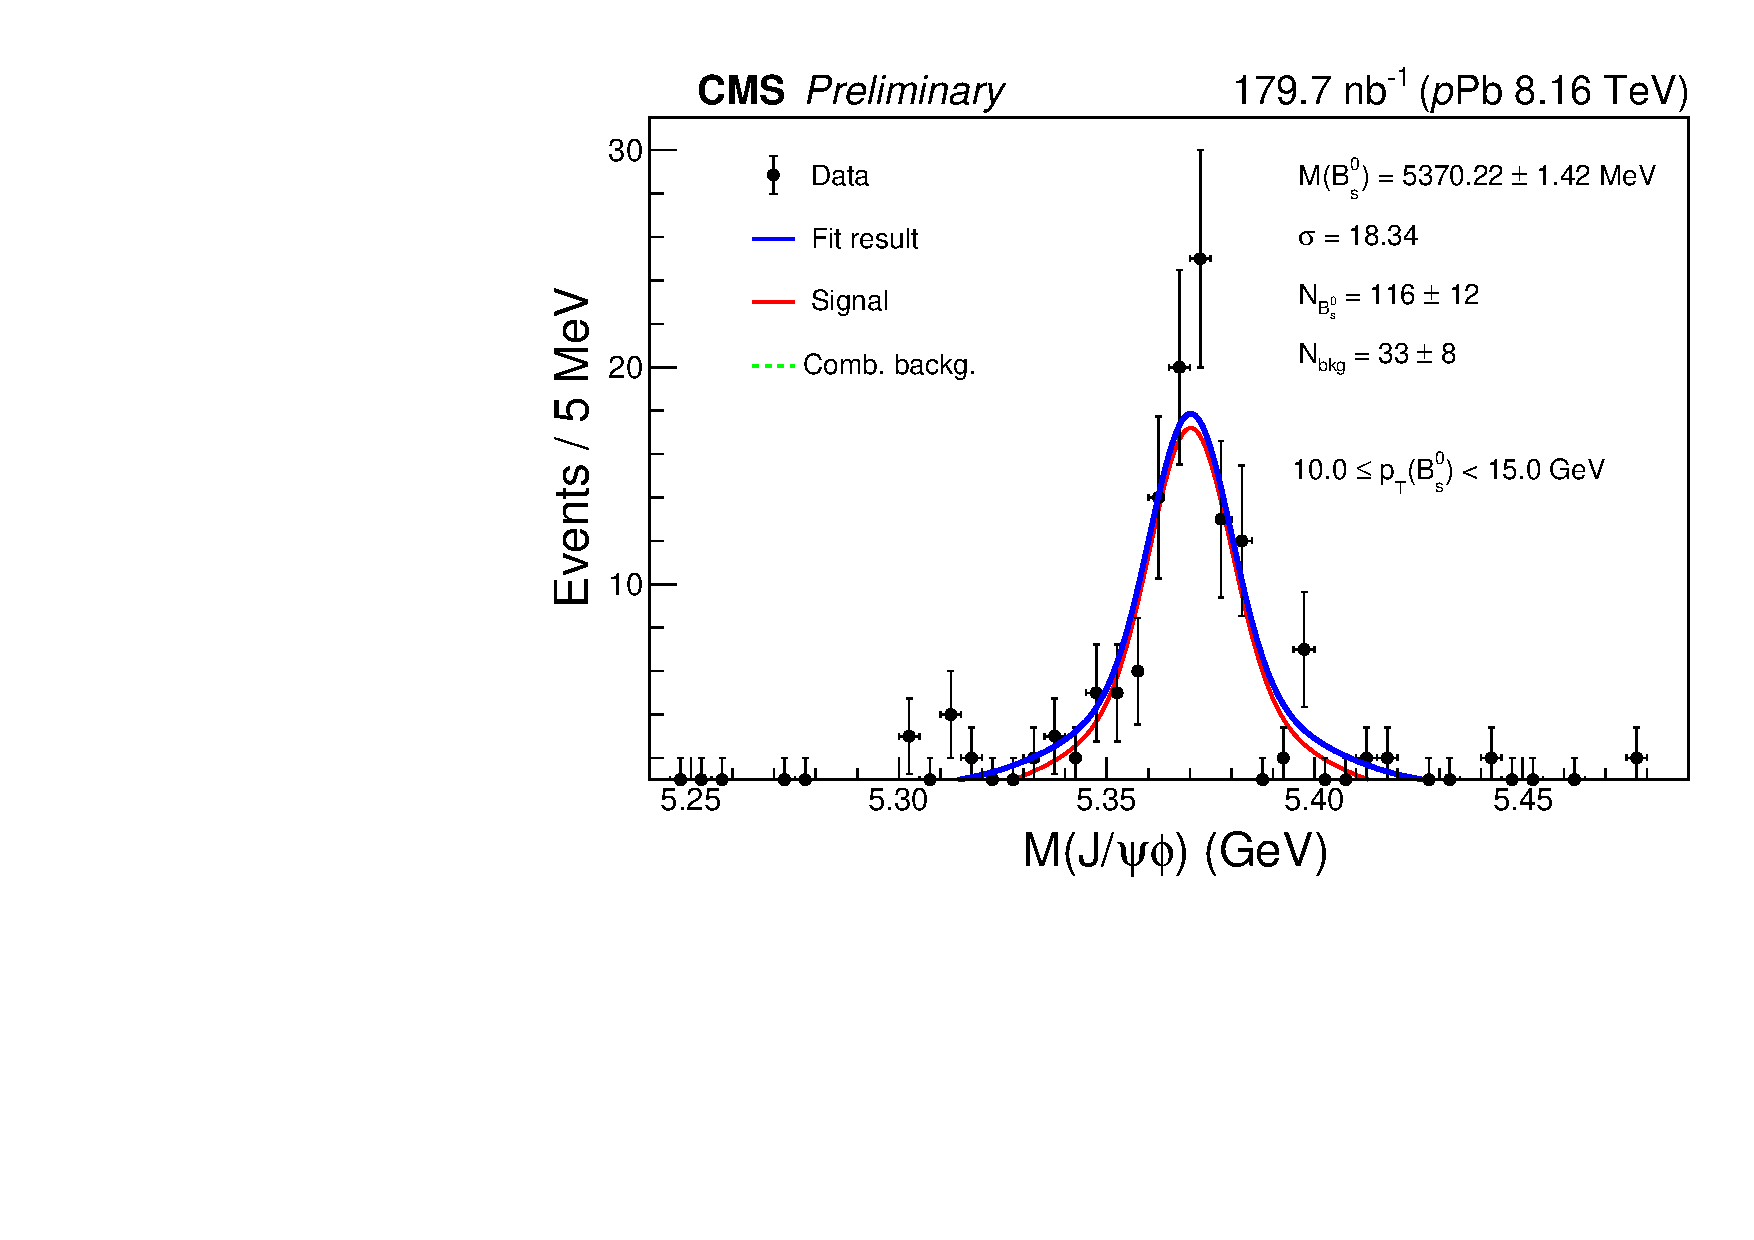
\includegraphics[width=\textwidth]{MainContent/Figs/mass/mass_BsFit_ptbins_sysbkg_10_15.PDF}
		\caption{}%
	\end{subfigure}
	\vskip\baselineskip
	\begin{subfigure}[b]{0.475\textwidth}
		\centering
		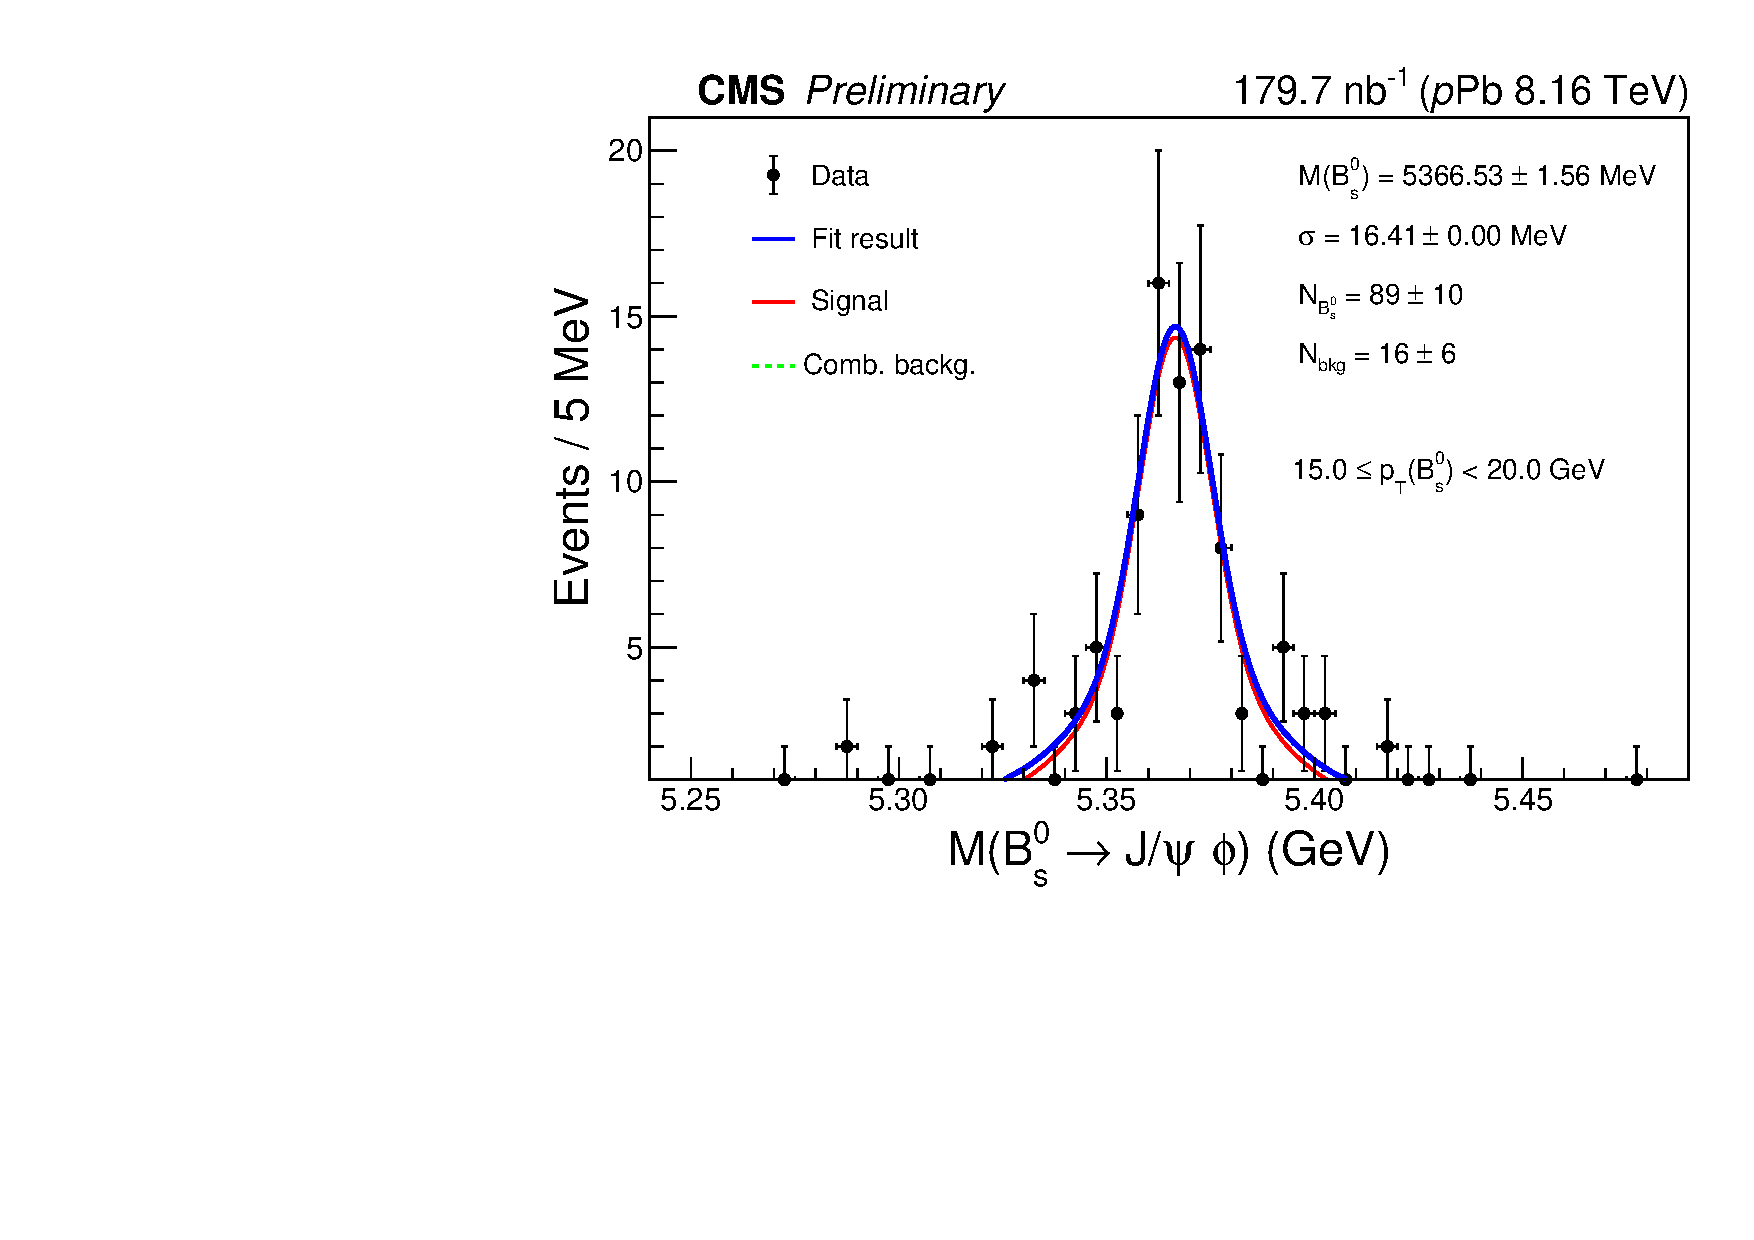
\includegraphics[width=\textwidth]{MainContent/Figs/mass/mass_BsFit_ptbins_sysbkg_15_20.PDF}
		\caption{}
	\end{subfigure}
	\hfill
	\begin{subfigure}[b]{0.475\textwidth}
		\centering
		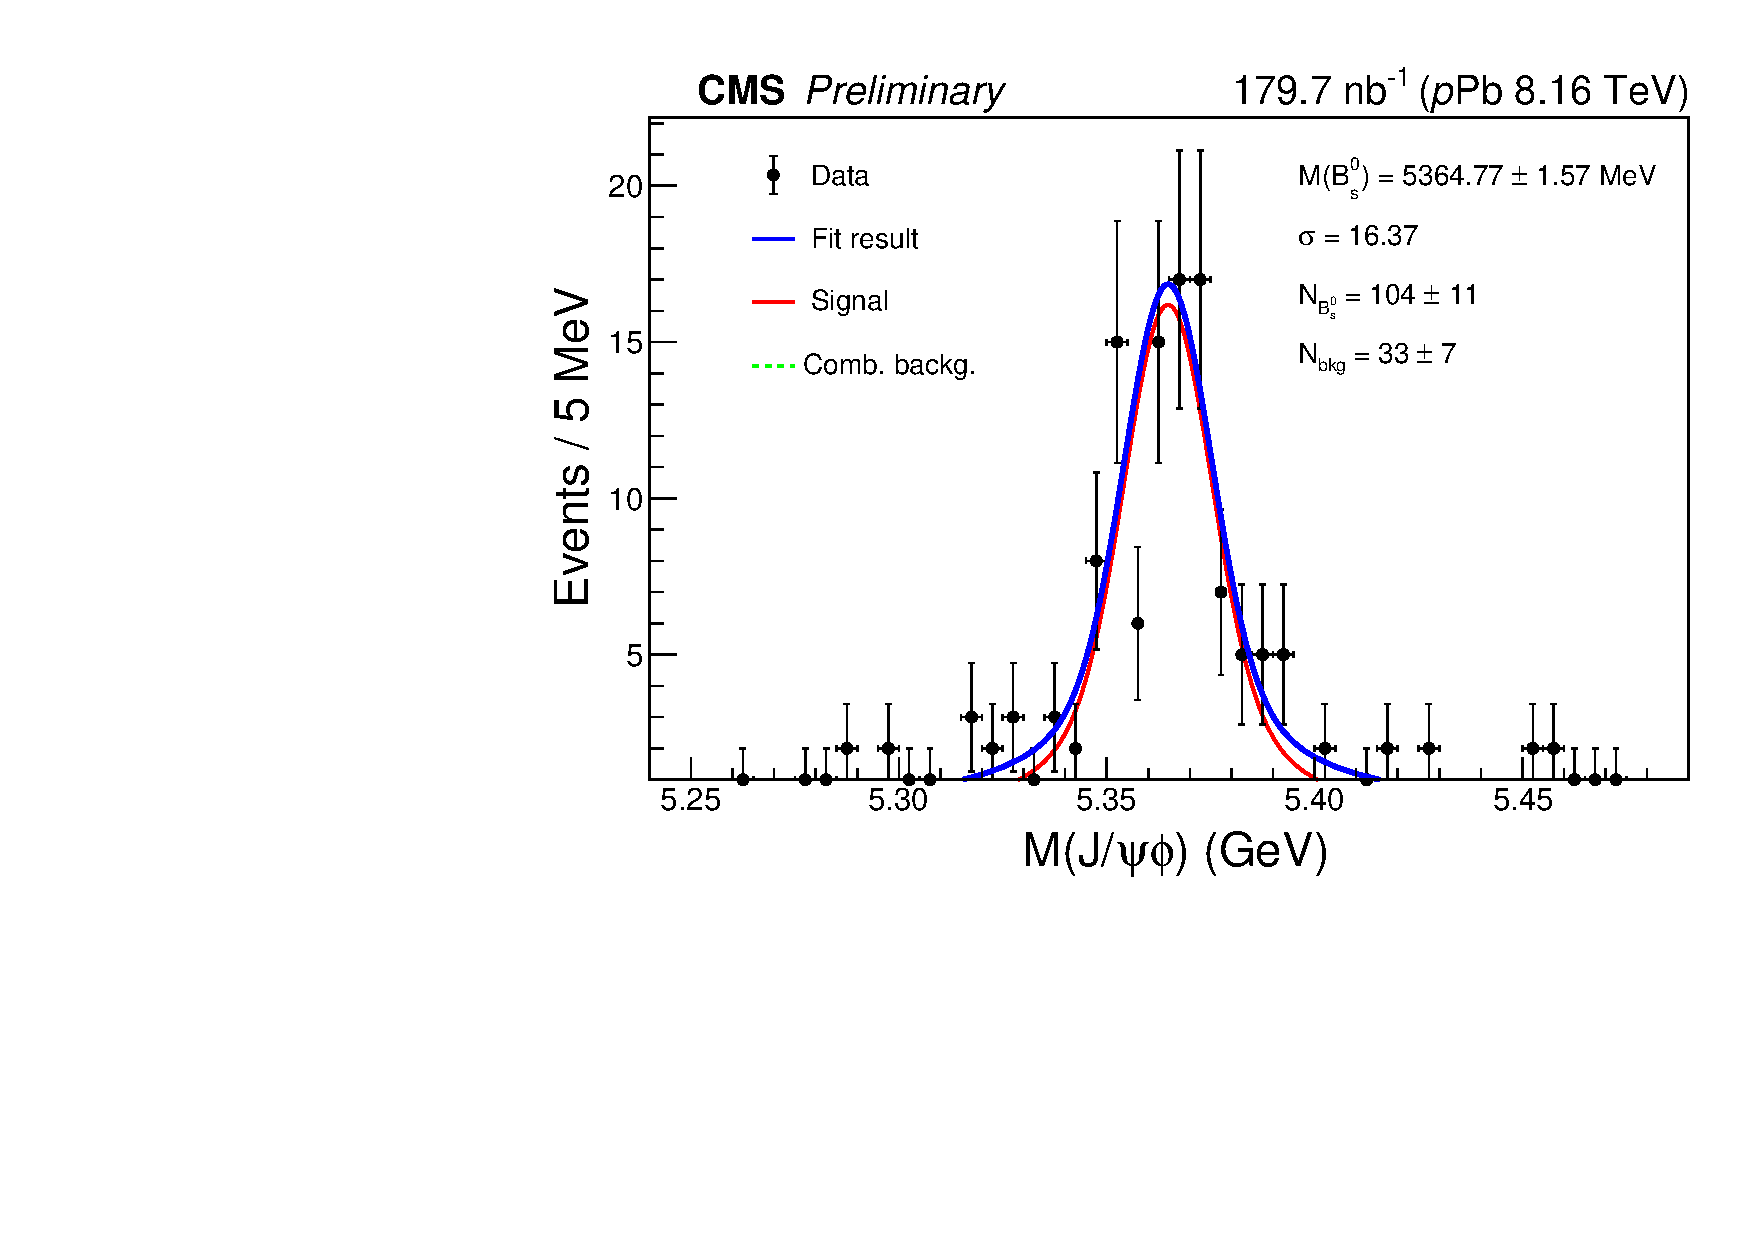
\includegraphics[width=\textwidth]{MainContent/Figs/mass/mass_BsFit_ptbins_sysbkg_20_50.PDF}
		\caption{}%
	\end{subfigure}
	\caption{Invariant mass spectra for $B^0_s$ meson reconstructed from the combined system $J/\psi \phi$ and considering a systematic model for background. Four intervals for the transverse momentum $p_T(B^0_s)$ have been considered.}
	\label{fig:mass_ptbins_sysbkg}
	%%%%%%%%%%%%%%%%%%%%%%%%%%%%%%%%%%%%second row
	
\end{figure}



\begin{figure*}
	\centering
	\begin{subfigure}[b]{0.7\textwidth}
		\centering
		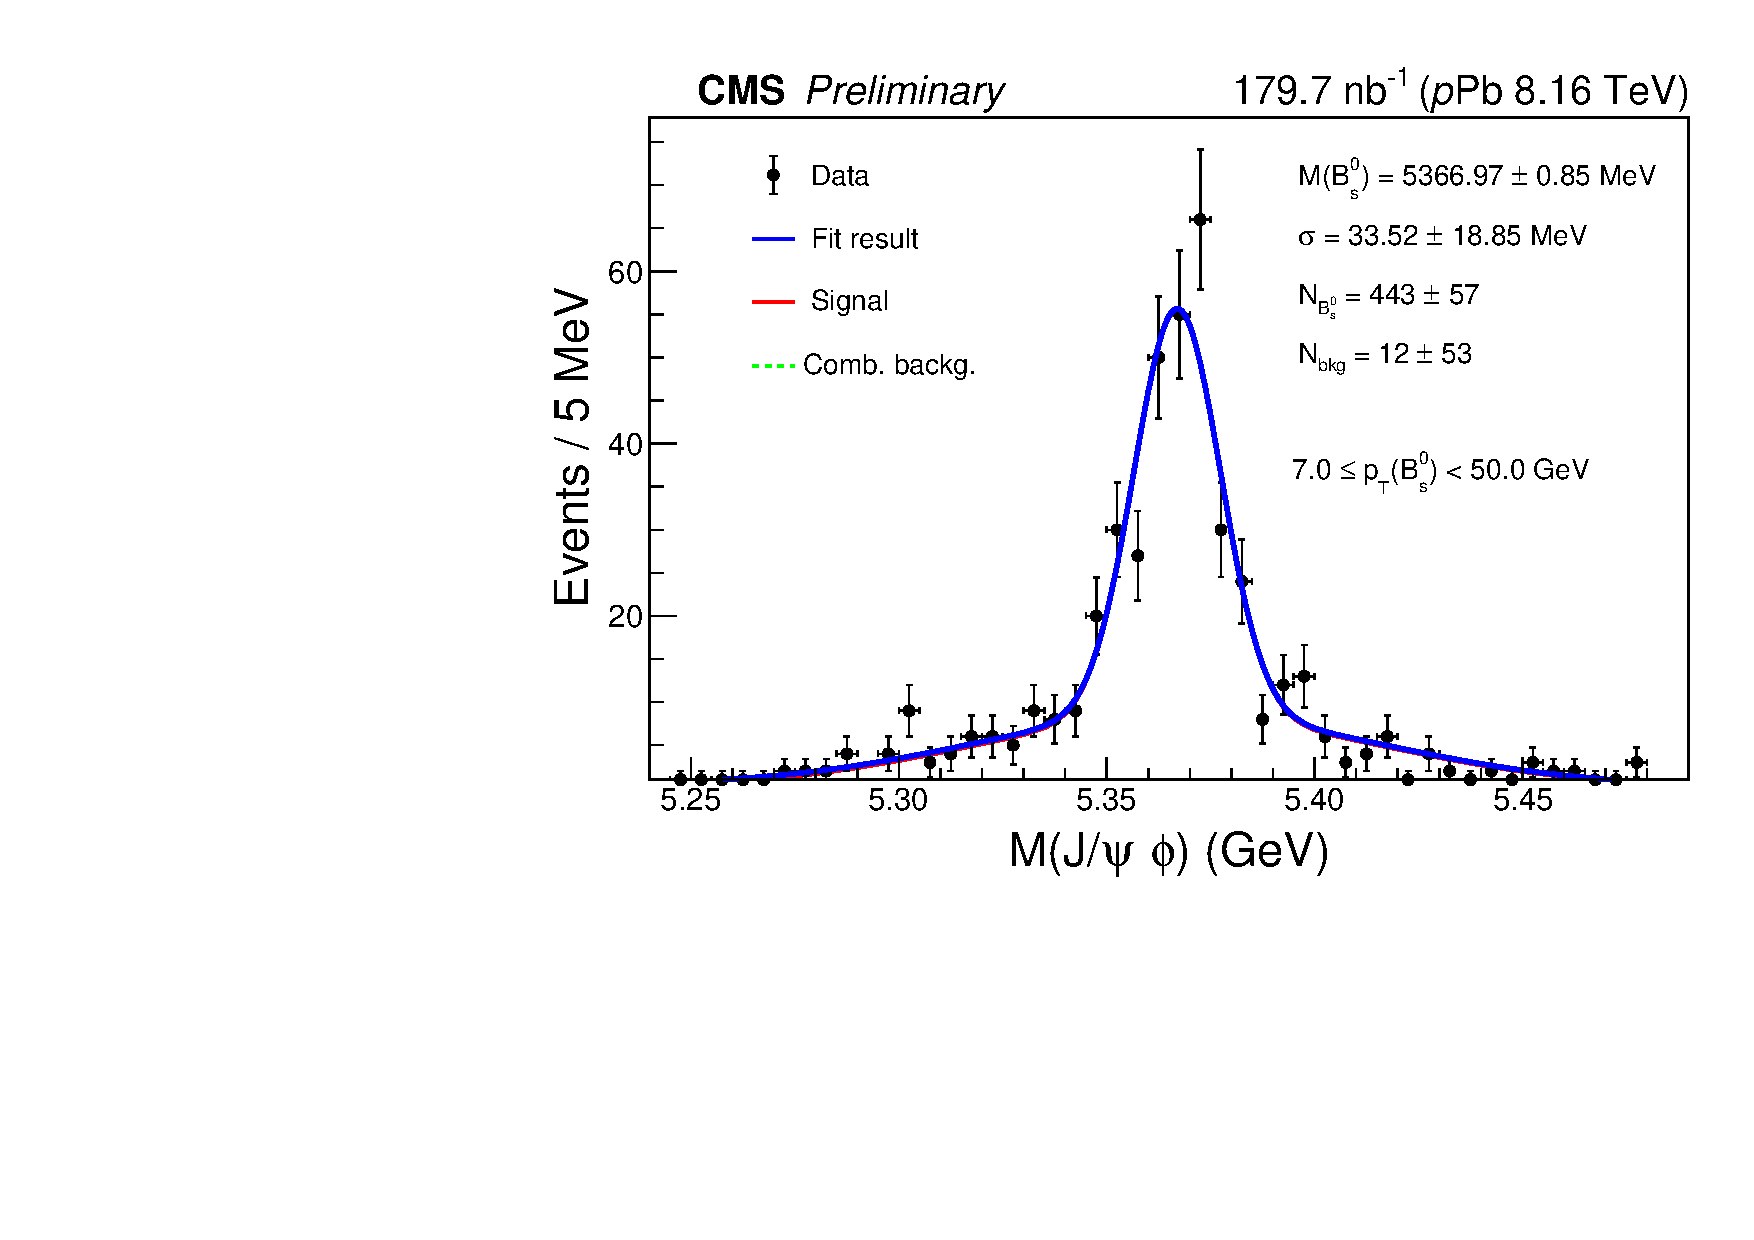
\includegraphics[width=\textwidth]{MainContent/Figs/mass/mass_BsFit_ptbins_syssig_7_50.PDF}
		\caption{}%
	\end{subfigure}
	\vskip\baselineskip
	\begin{subfigure}[b]{0.7\textwidth}
		\centering
		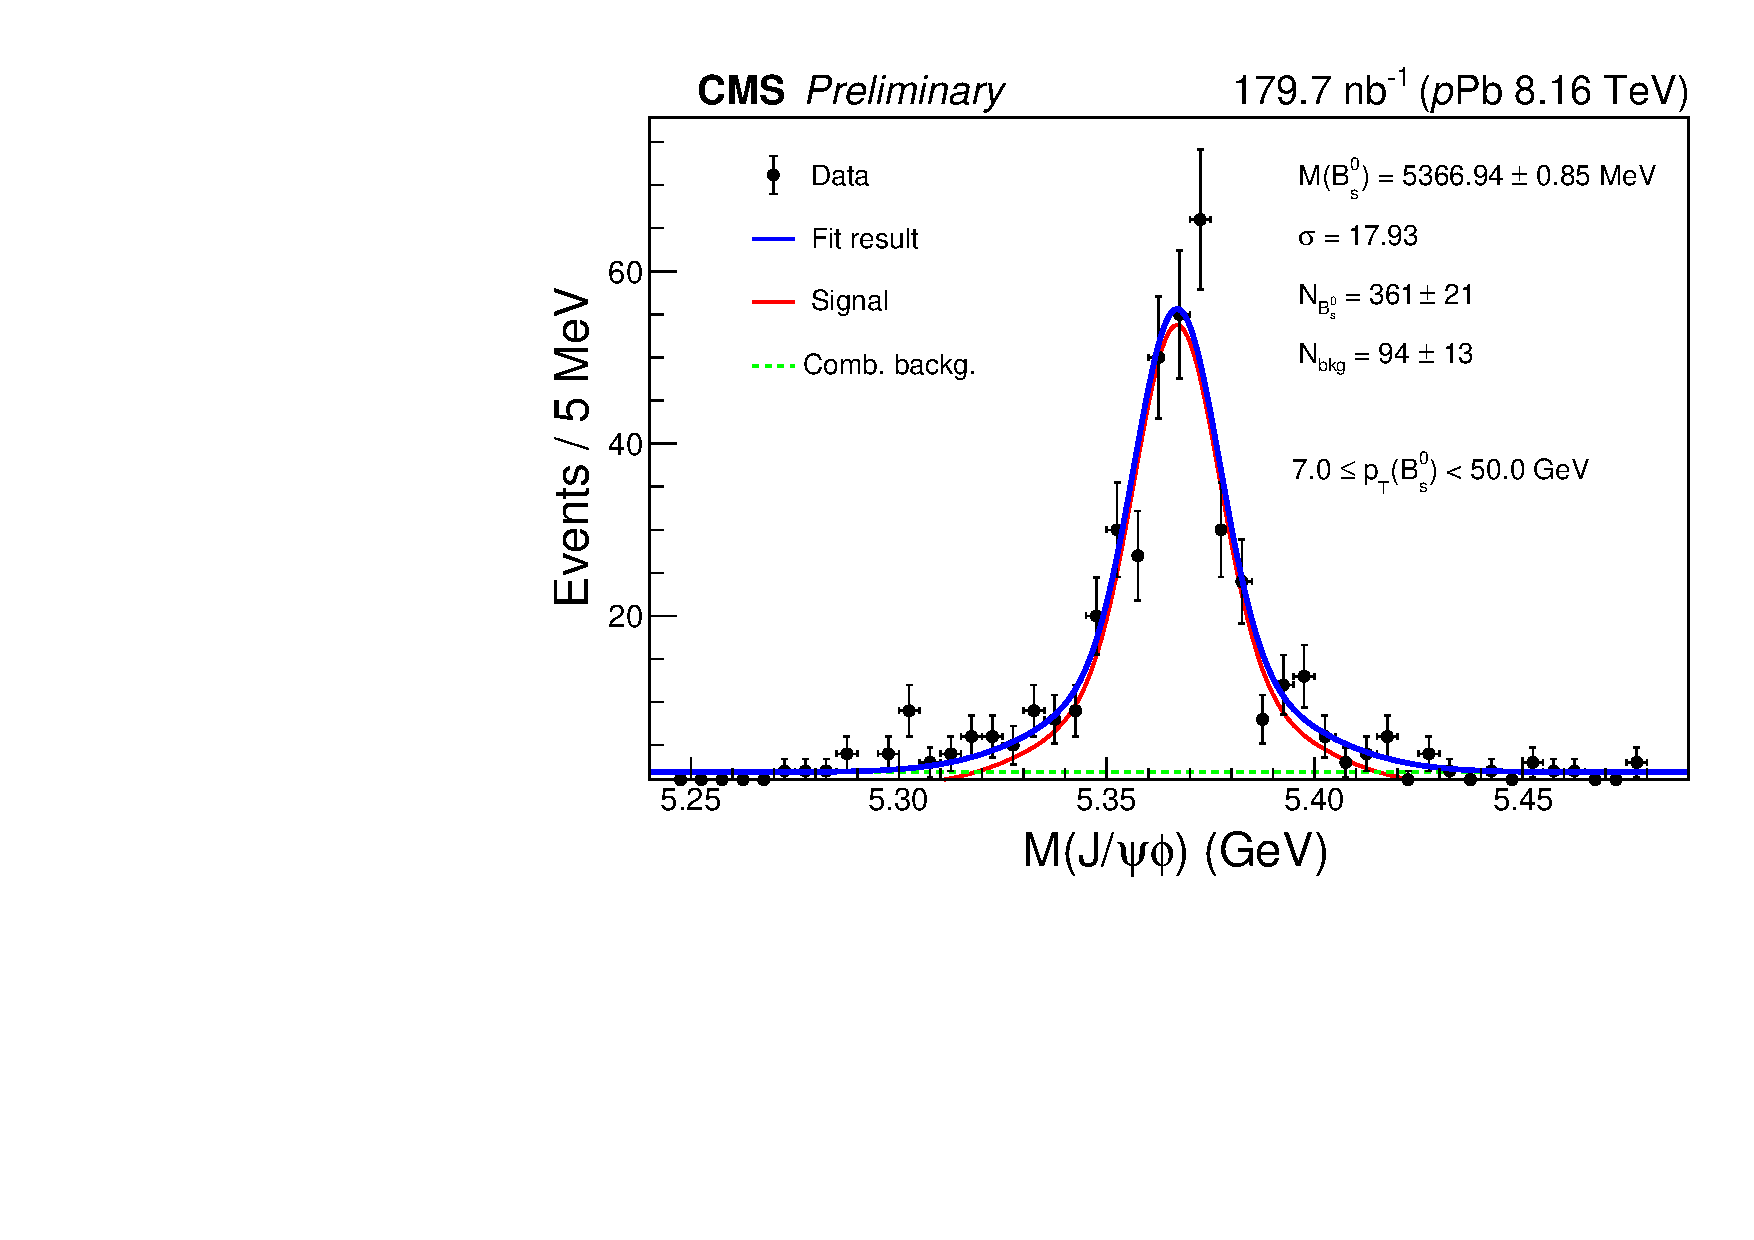
\includegraphics[width=\textwidth]{MainContent/Figs/mass/mass_BsFit_ptbins_sysbkg_7_50.PDF}
		\caption{}%
	\end{subfigure}
	\caption{Invariant mass spectra for the $B^0_s$ meson reconstructed from the combined system $J/\psi \phi$. a) corresponds to the systematic model for signal b) for background}
	\label{fig:mass_ptbins_sys}
\end{figure*}

\begin{figure}[htp!]
	\centering
	\centering
	\begin{subfigure}[b]{0.475\textwidth}
		\centering
		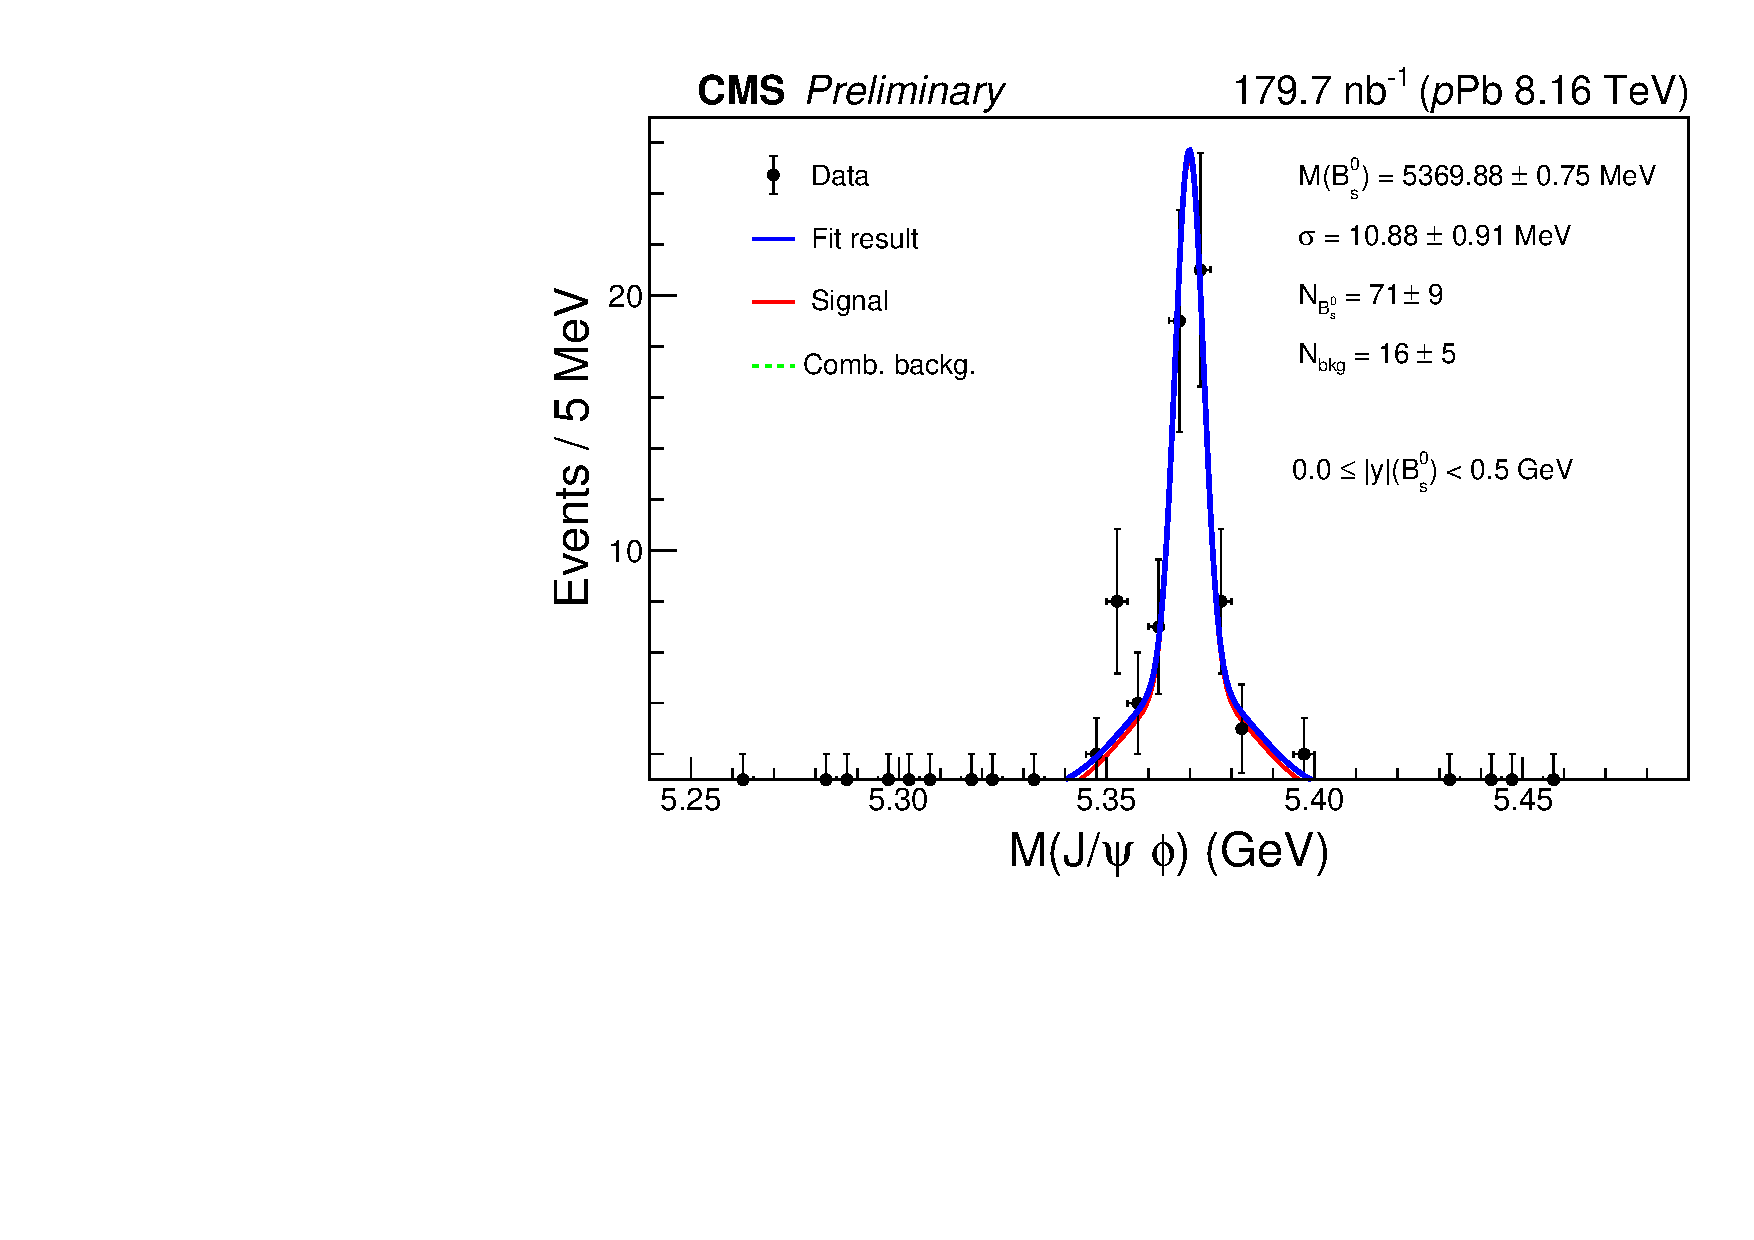
\includegraphics[width=\textwidth]{MainContent/Figs/mass/mass_BsFit_ybins_syssig_0.0_0.5.PDF}
		\caption{}%
	\end{subfigure}
	\hfill
	\begin{subfigure}[b]{0.475\textwidth}
		\centering
		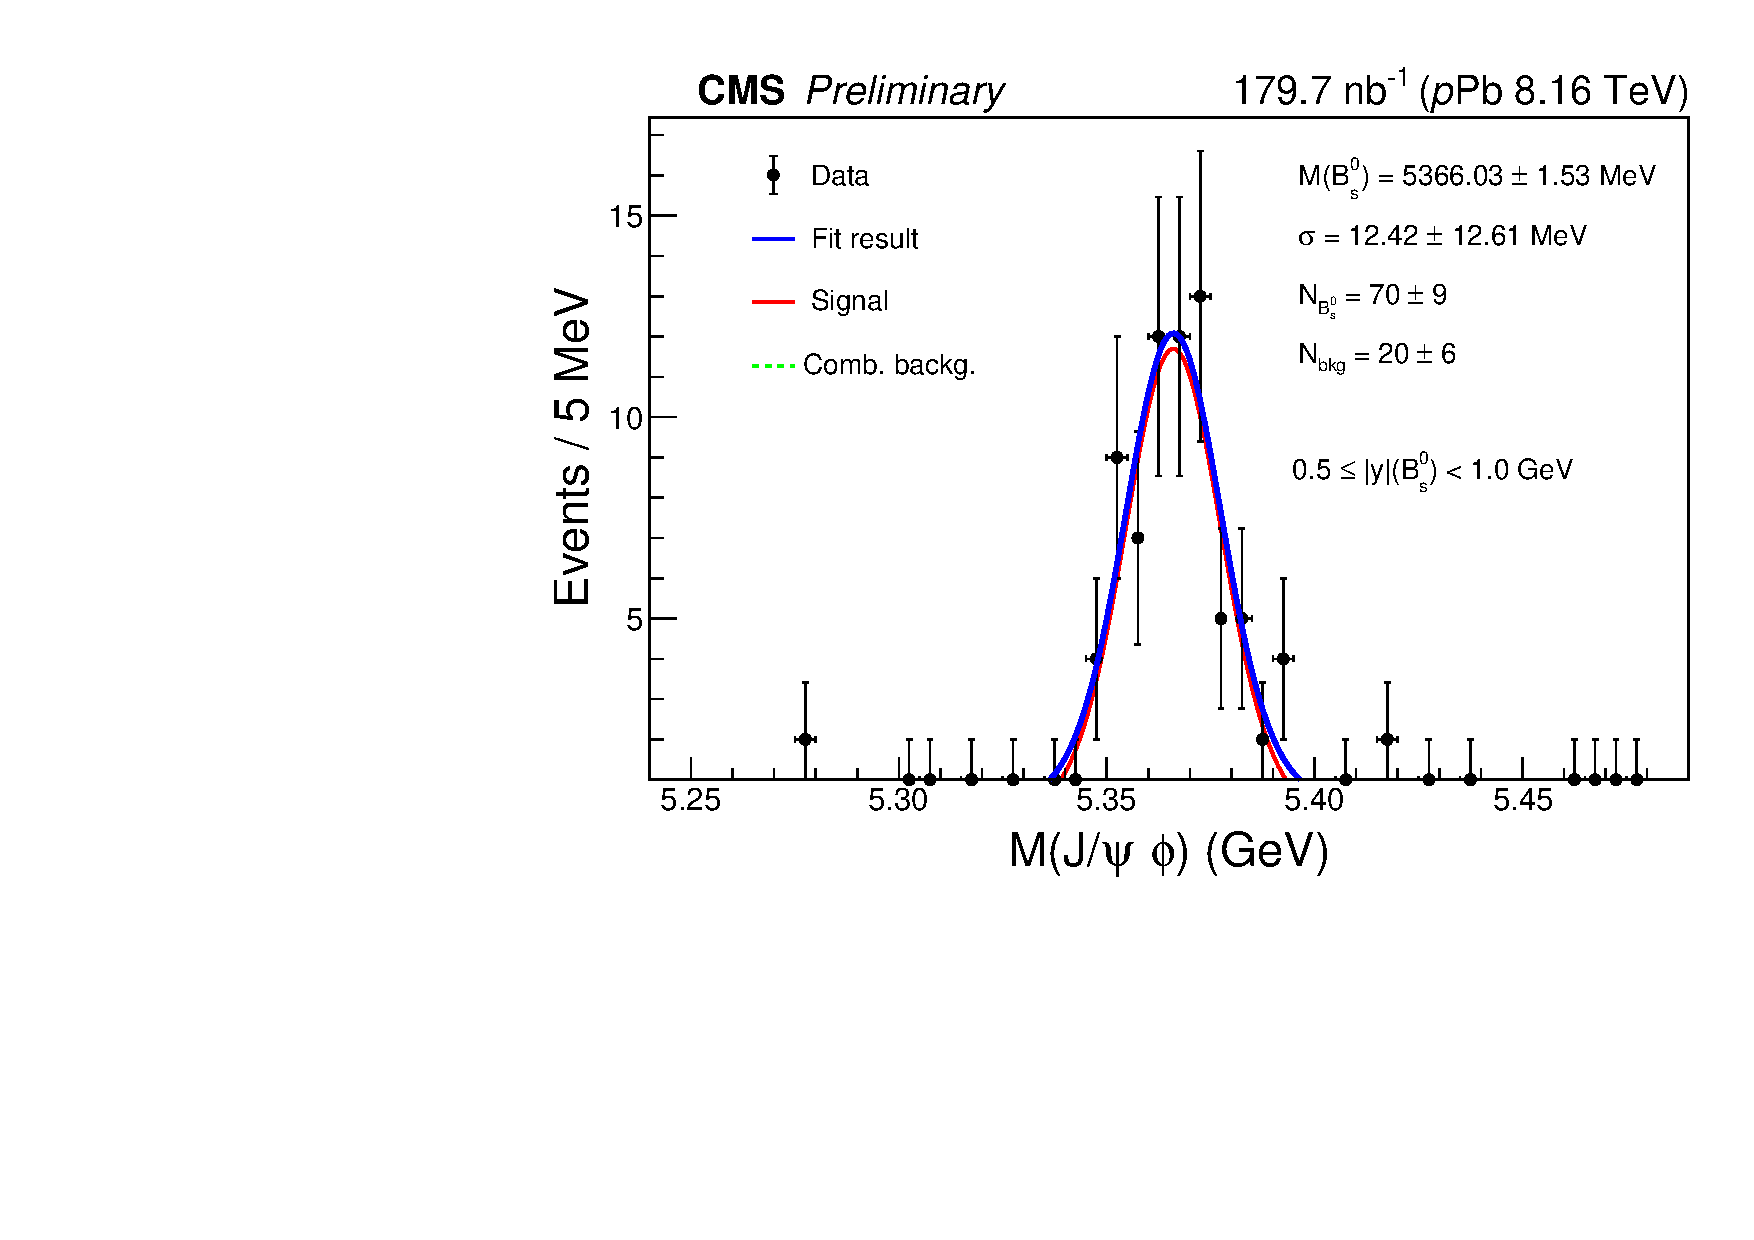
\includegraphics[width=\textwidth]{MainContent/Figs/mass/mass_BsFit_ybins_syssig_0.5_1.0.PDF}
		\caption{}%
		
	\end{subfigure}
	\vskip\baselineskip
	\begin{subfigure}[b]{0.475\textwidth}
		\centering
		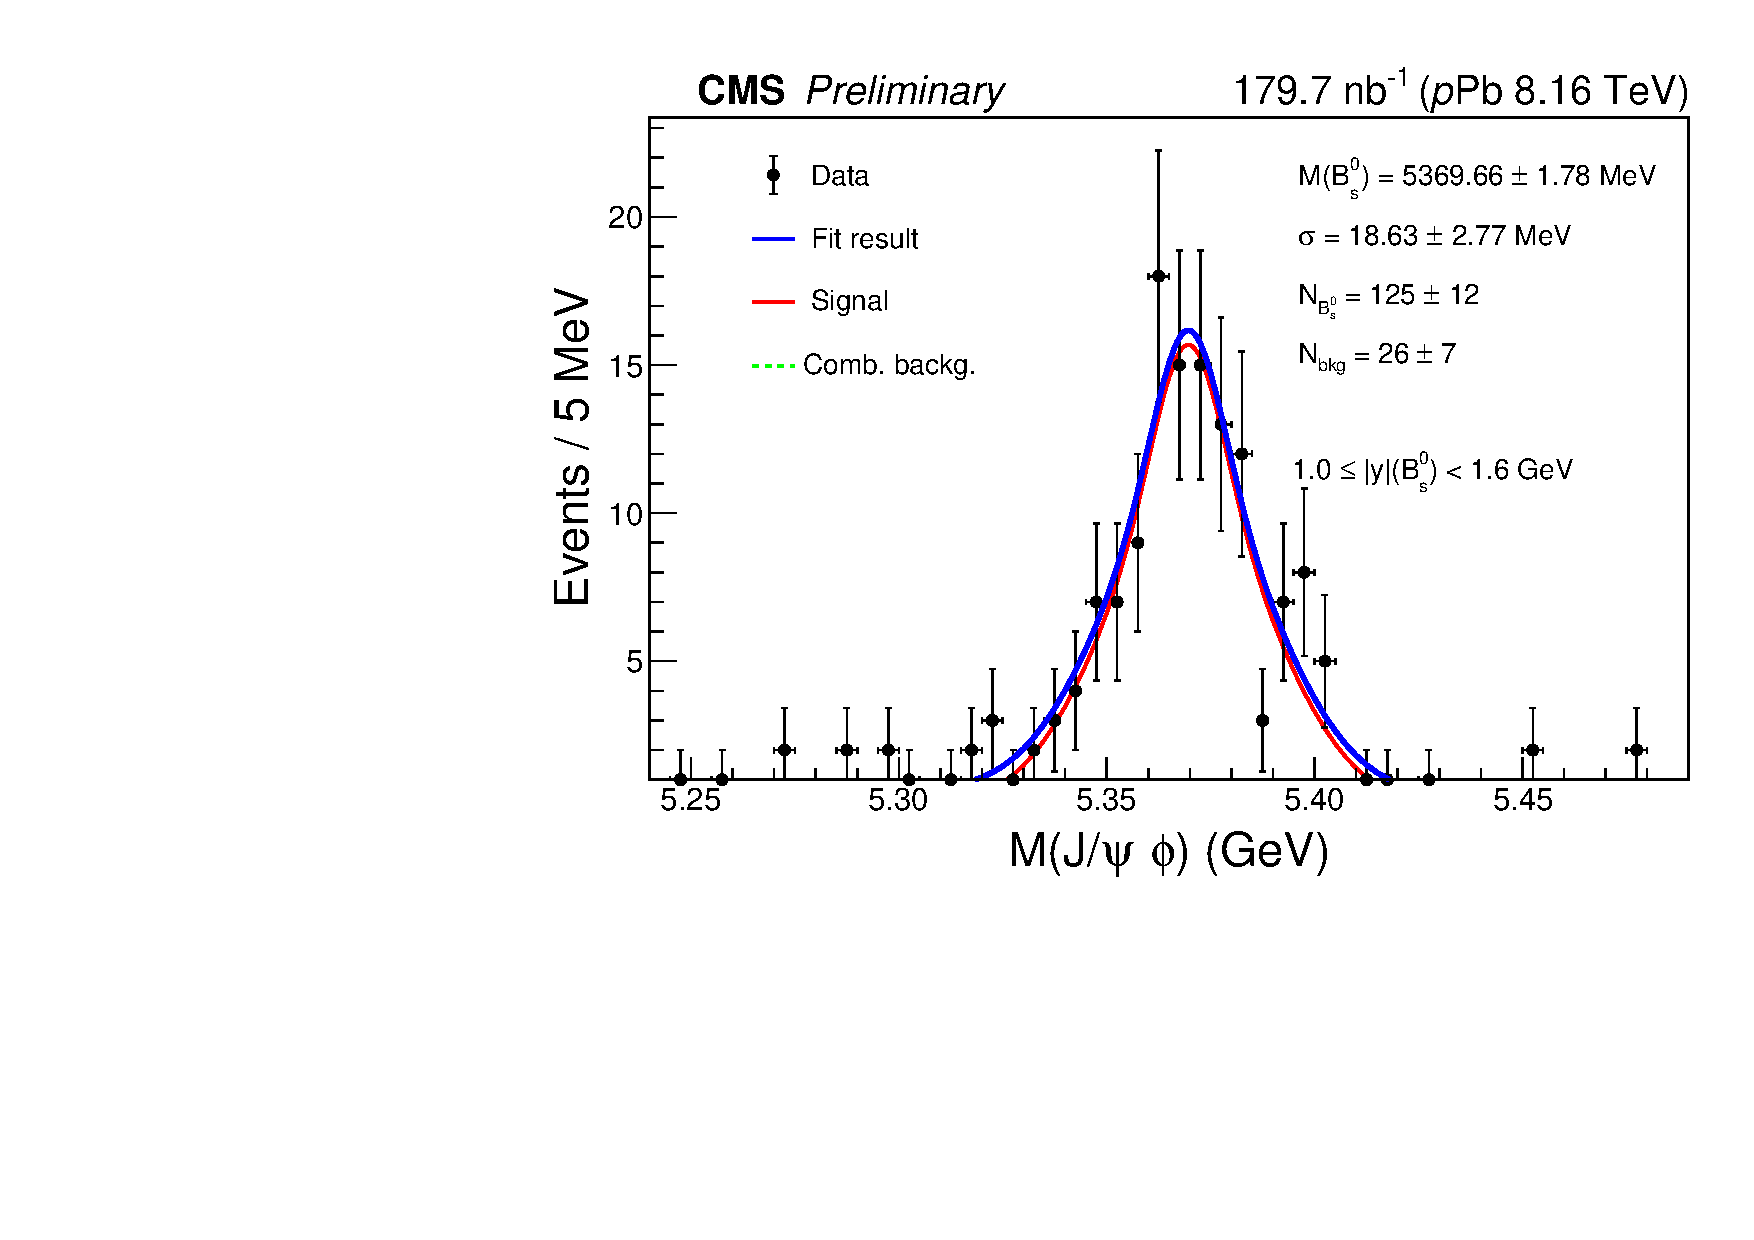
\includegraphics[width=\textwidth]{MainContent/Figs/mass/mass_BsFit_ybins_syssig_1.0_1.6.PDF}
		\caption{}
	\end{subfigure}
	\hfill
	\begin{subfigure}[b]{0.475\textwidth}
		\centering
		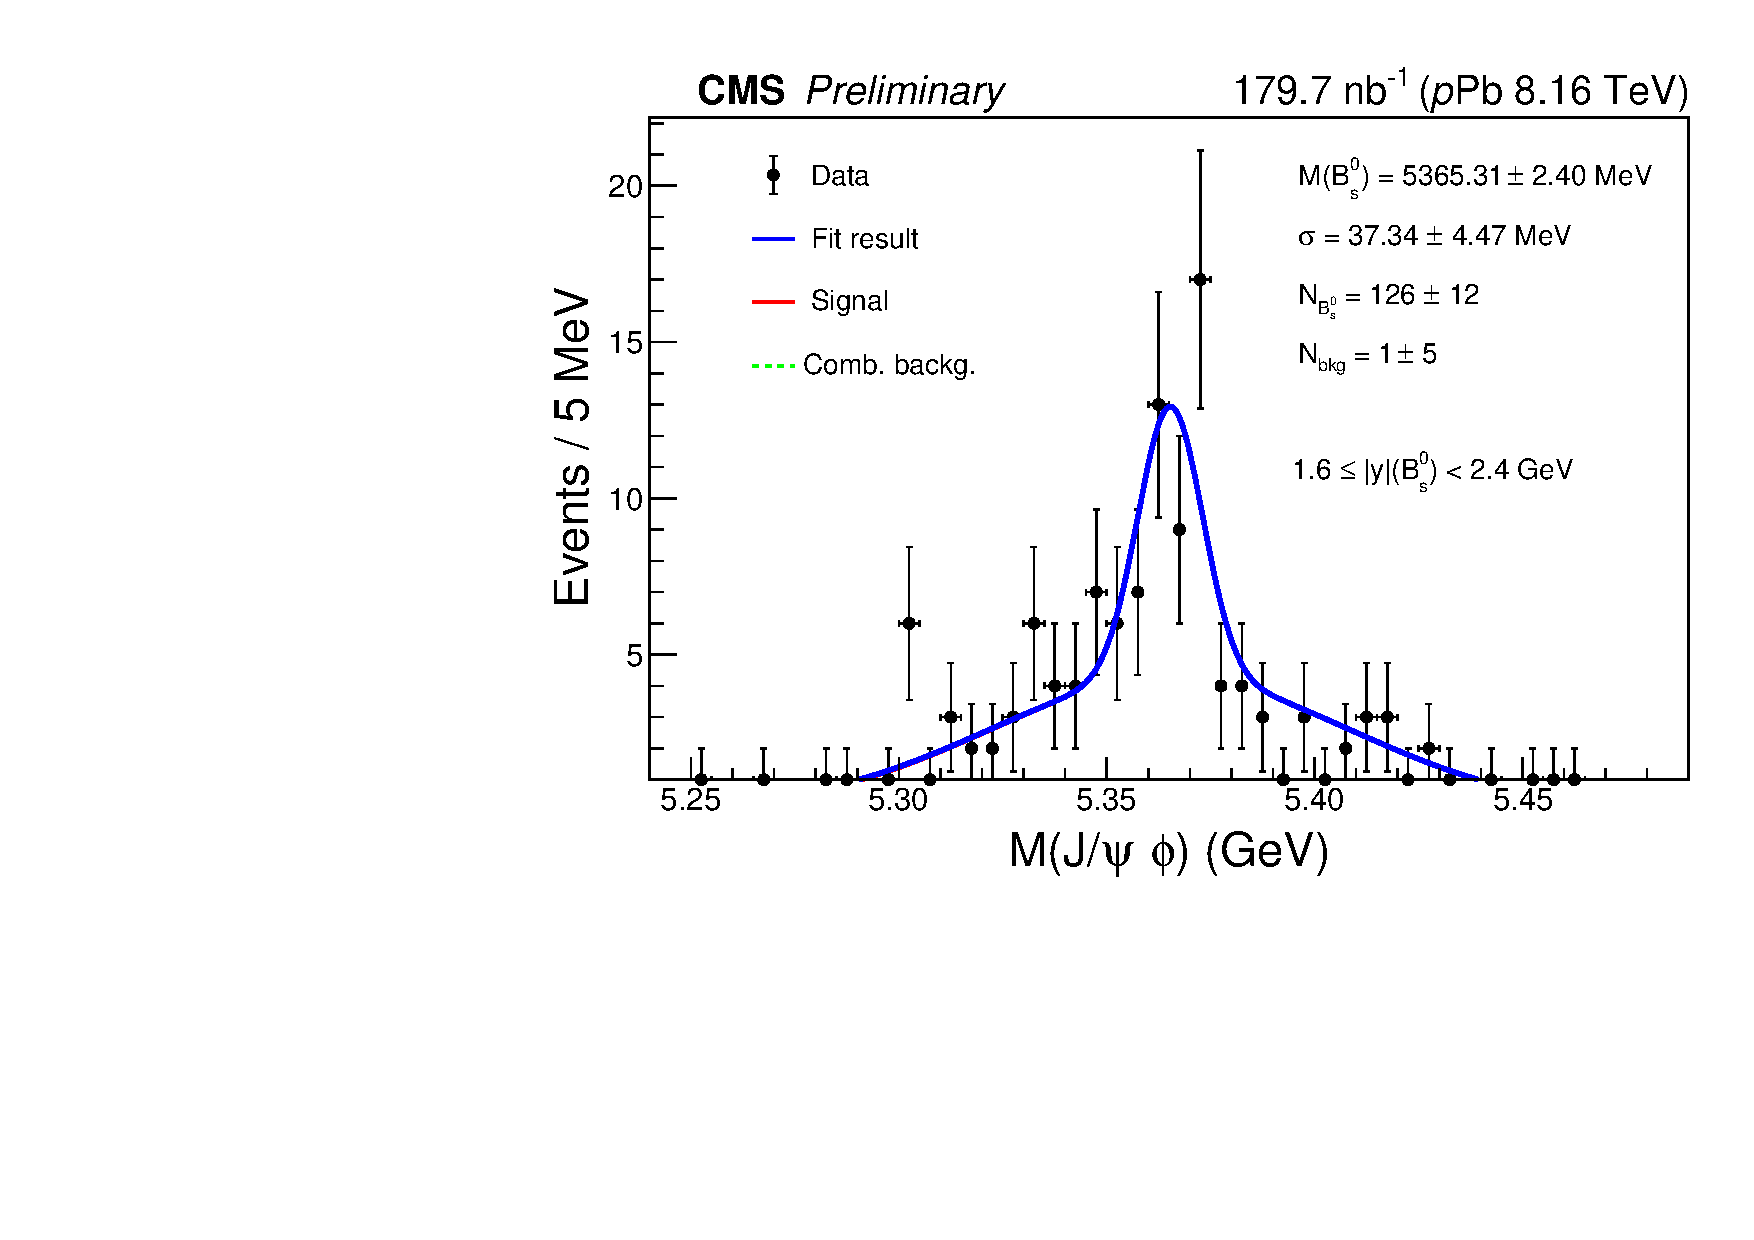
\includegraphics[width=\textwidth]{MainContent/Figs/mass/mass_BsFit_ybins_syssig_1.6_2.4.PDF}
		\caption{}%
	\end{subfigure}
	\caption{Invariant mass spectra for $B^0_s$ meson reconstructed from the combined system $J/\psi \phi$ and considering a systematic model for signal. Four intervals for the rapidity $|y|(B^0_s)$ have been considered.}
	\label{fig:mass_ybins_syssig}
	%%%%%%%%%%%%%%%%%%%%%%%%%%%%%%%%%%%%second row
	
\end{figure}


\begin{figure}[htp!]
	\centering
	\centering
	\begin{subfigure}[b]{0.475\textwidth}
		\centering
		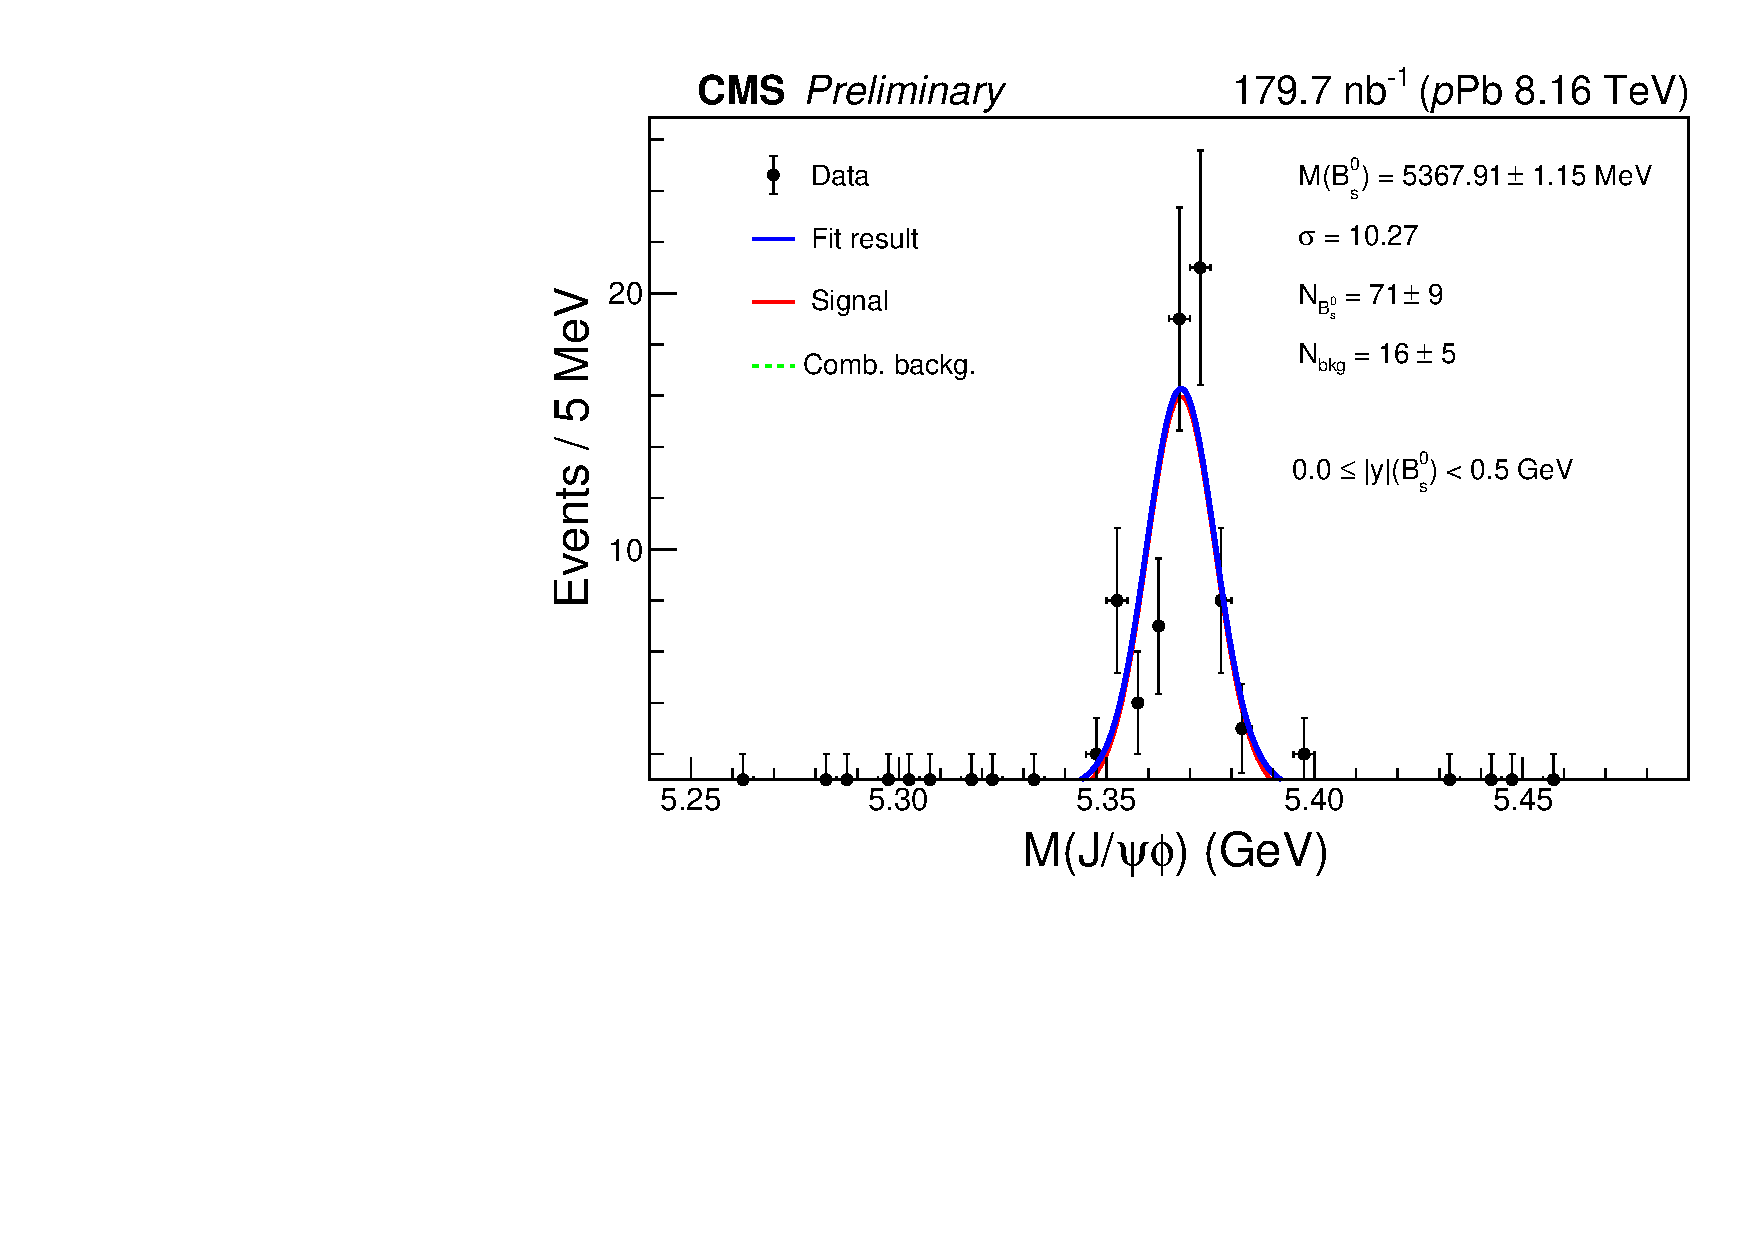
\includegraphics[width=\textwidth]{MainContent/Figs/mass/mass_BsFit_ybins_sysbkg_0.0_0.5.PDF}
		\caption{}%
	\end{subfigure}
	\hfill
	\begin{subfigure}[b]{0.475\textwidth}
		\centering
		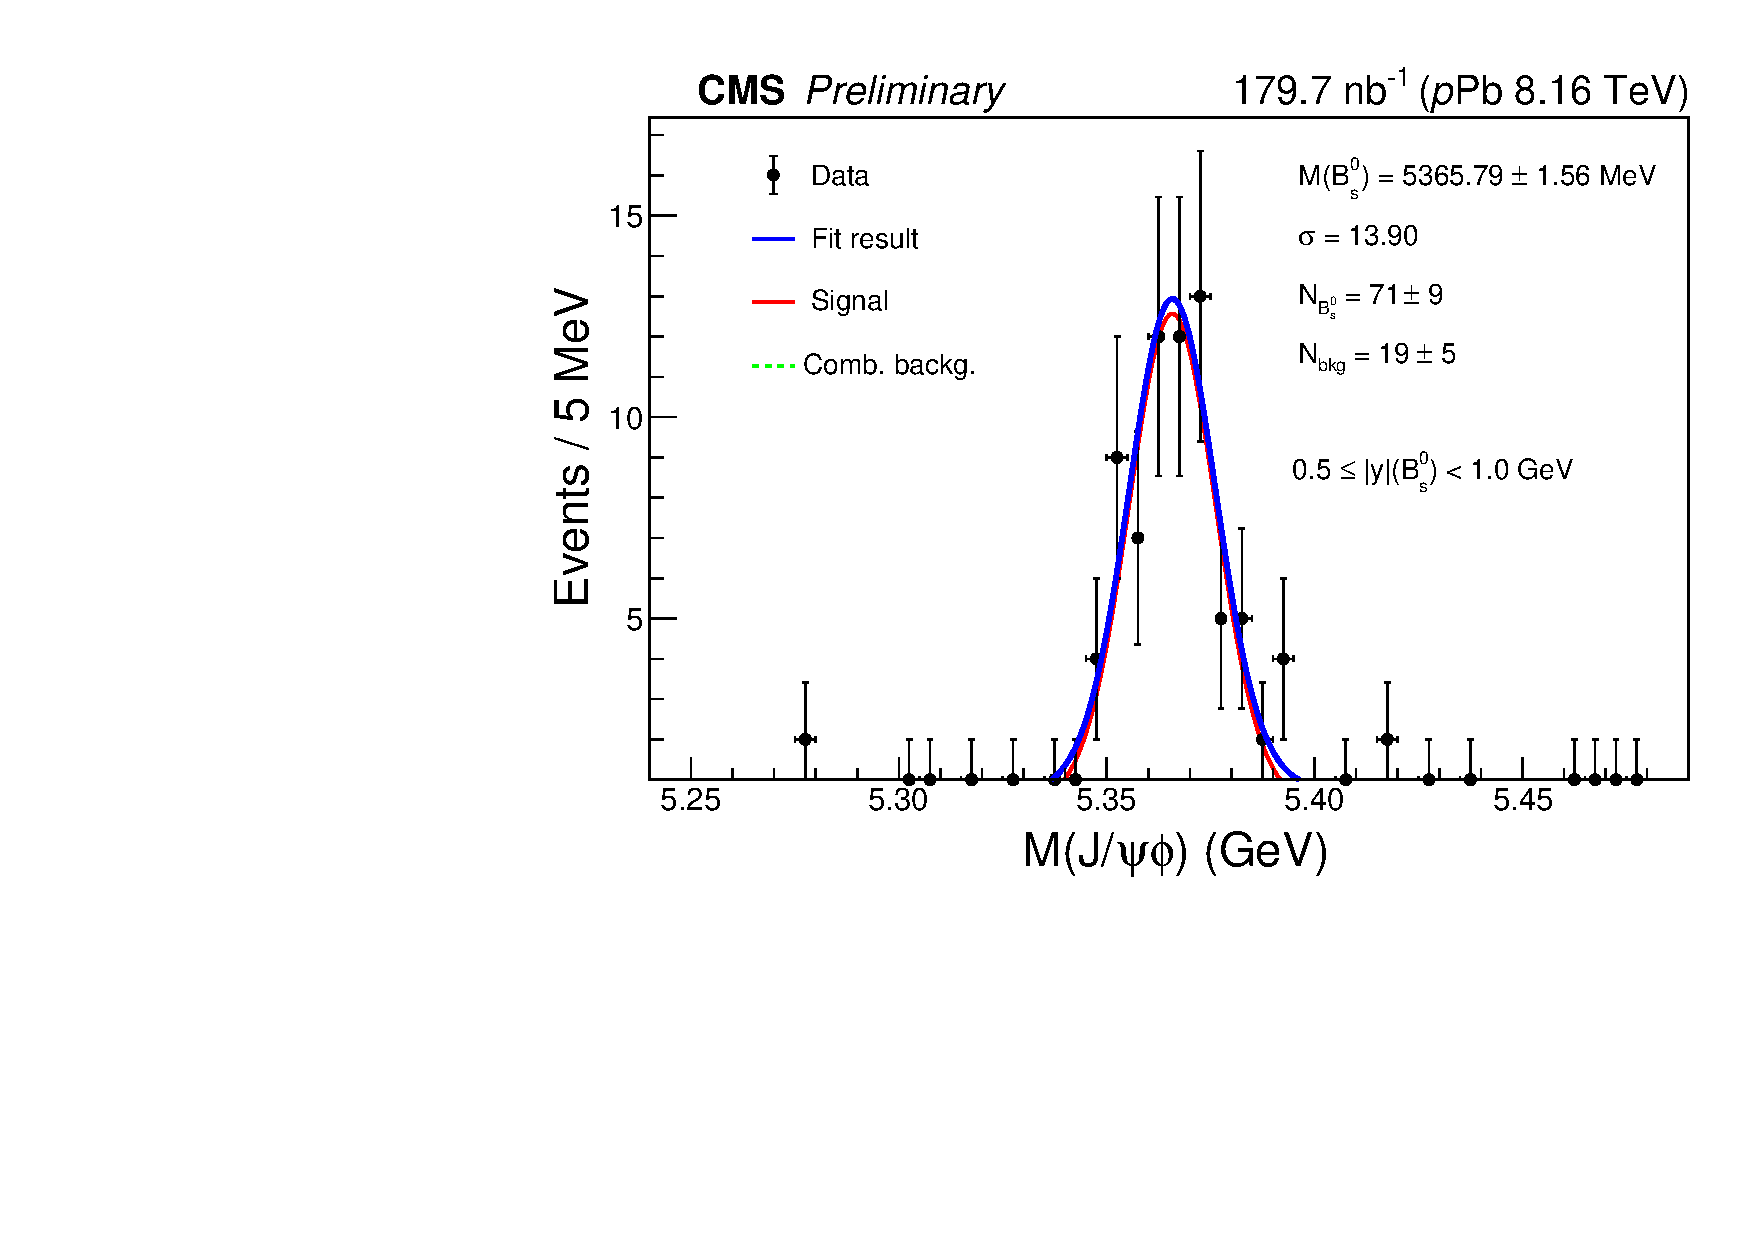
\includegraphics[width=\textwidth]{MainContent/Figs/mass/mass_BsFit_ybins_sysbkg_0.5_1.0.PDF}
		\caption{}%
		
	\end{subfigure}
	\vskip\baselineskip
	\begin{subfigure}[b]{0.475\textwidth}
		\centering
		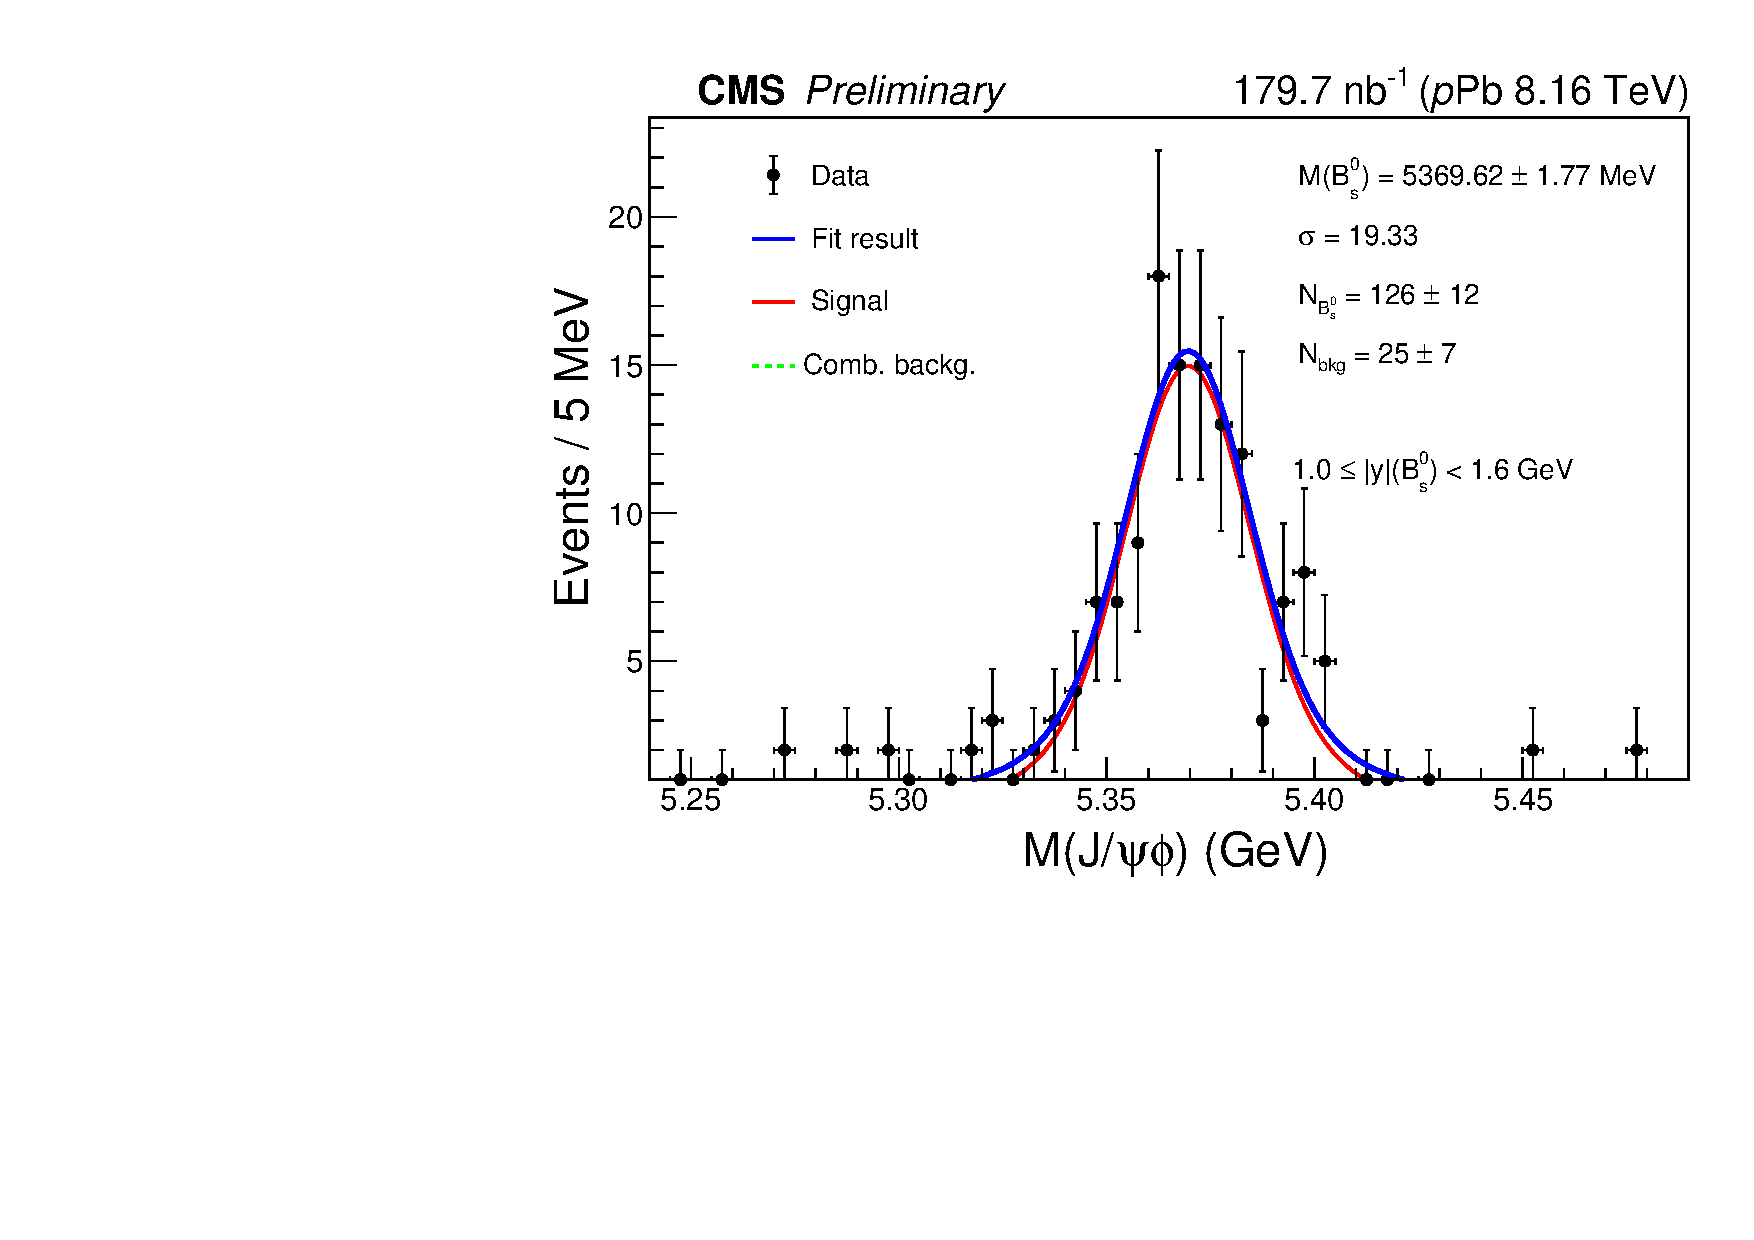
\includegraphics[width=\textwidth]{MainContent/Figs/mass/mass_BsFit_ybins_sysbkg_1.0_1.6.PDF}
		\caption{}
	\end{subfigure}
	\hfill
	\begin{subfigure}[b]{0.475\textwidth}
		\centering
		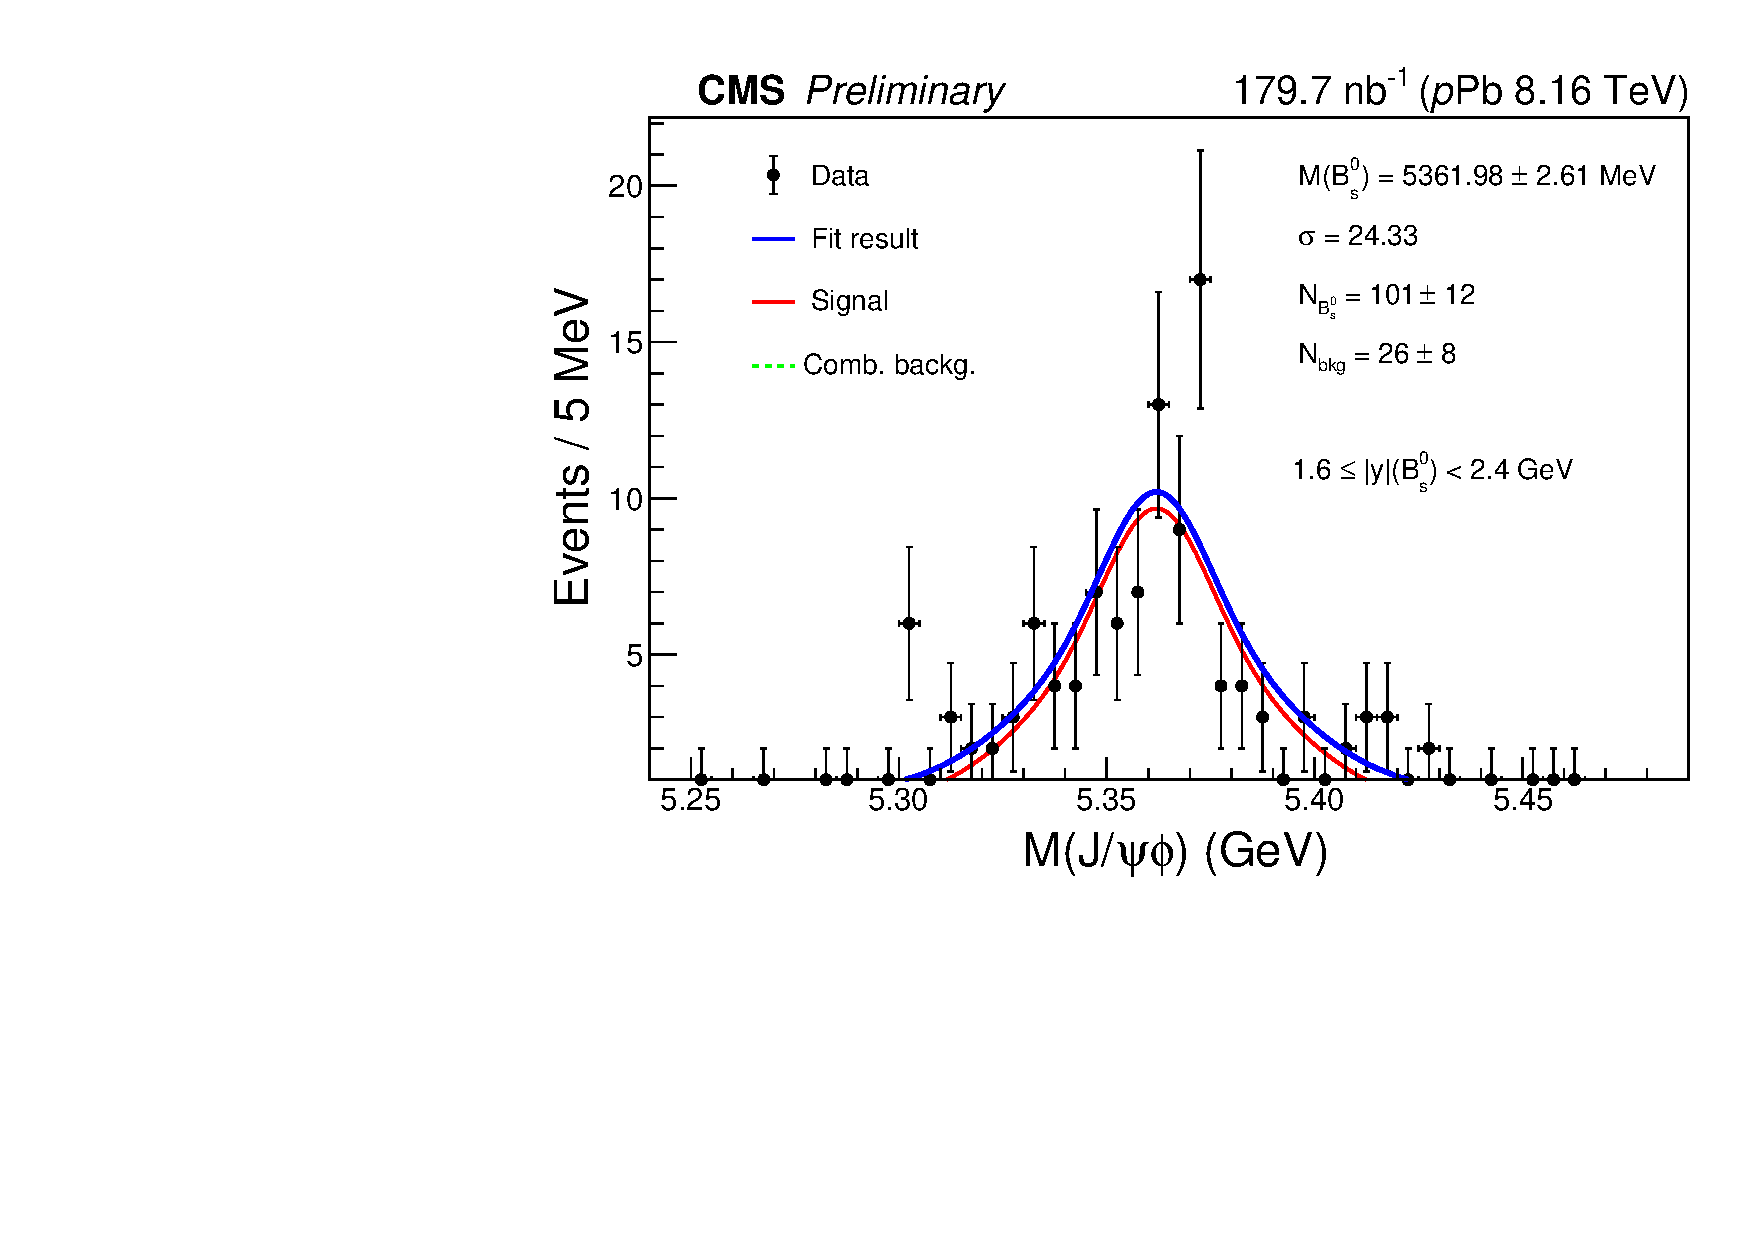
\includegraphics[width=\textwidth]{MainContent/Figs/mass/mass_BsFit_ybins_sysbkg_1.6_2.4.PDF}
		\caption{}%
	\end{subfigure}
	\caption{Invariant mass spectra for $B^0_s$ meson reconstructed from the combined system $J/\psi \phi$ and considering a systematic model for background. Four intervals for the rapidity $|y|(B^0_s)$ have been considered.}
	\label{fig:mass_ybins_sysbkg}
	%%%%%%%%%%%%%%%%%%%%%%%%%%%%%%%%%%%%second row
	
\end{figure}


\cleardoublepage
\subsection{Efficiency}

\subsubsection{MC size}
The uncertainties of the ratios defined for the acceptance and efficiency, $\delta \alpha$ and $\delta \epsilon$ are statistical. However, due to the finite size of the number of Monte Carlo samples used for reconstruction, they turn into systematic uncertainties when considering the differential cross-section. For practical purposes, the uncertainty of the total efficiency $\delta(\alpha \cdot \epsilon)$ is used instead of the individual uncertainties.


\subsubsection{Track}

The uncertainty in the efficiency of reconstruction of the tracks ($K^{+}K^{-}$) is considered a systematic uncertainty. In this paper, the value reported by \cite{cms2018tracking} will be used as the track efficiency uncertainty: $2.4\%$.

In the table \ref{table:Systematics}, the statistical and the systematic uncertainties considered for the cross-section are presented for each of the $p_T$ bins and in table \ref{table:Systematics_y} for the $|y|$ bins.
\begin{table}[htbp] \begin{center}\begin{tabular}{|c|c|c|c|c|c|c|}\hline$\mathbf{p_T}$    &  $\mathbf{N_{B_s^{0}}} $    &  $\mathbf{N_{B_s^{0}}} $  & \textbf{MC}   & \textbf{Tracking}  & \textbf{Total Systematic}  & \textbf{Statistical} \\\textbf{(GeV)}   & \textbf{signal}   & \textbf{bkg}    & \textbf{size} &           & \textbf{uncertainty} ($\mathbf{\%}$) & \textbf{uncertainty} ($\mathbf{\%}$) \\\hline{[}7, 10{)}  &  10.0  &  0.1 &  4.6  &  2.4 &  11.3 &  14.9 \\{[}10, 15{)}  &  8.1  &  0.1 &  2.5  &  2.4 &  8.8 &  10.2 \\{[}15, 20{)}  &  12.3  &  0.1 &  2.8  &  2.4 &  12.9 &  11.5 \\{[}20, 50{)}  &  26.0  &  0.0 &  2.7  &  2.4 &  26.2 &  10.8 \\\hline\end{tabular}\caption{Systematic uncertainties on  ${\frac{d \sigma}{dp_T}}$ from alternative fitting strategies described in the text. The total systematic uncertainty is the sum in quadrature of the individual uncertainties. Statistical uncertainty is show too.}\label{table:Systematics}\end{center}\end{table}

\begin{table}[htbp] \begin{center}\begin{tabular}{|c|c|c|c|c|c|c|}\hline$\mathbf{|y|}$    &  $\mathbf{N_{B_s^{0}}} $    &  $\mathbf{B_s^{0}} $  & \textbf{MC}   & \textbf{Tracking}  & \textbf{Total Systematic}  & \textbf{Statistical} \\\textbf{(GeV)}   & \textbf{signal}   & \textbf{bkg}    & \textbf{size} &           & \textbf{uncertainty} ($\mathbf{\%}$) & \textbf{uncertainty} ($\mathbf{\%}$) \\\hline{[}0.0, 0.5{)}  &  0.1  &  0.1 &  3.2  &  2.4 &  4.0 &  12.3 \\{[}0.5, 1.0{)}  &  2.3  &  0.4 &  3.1  &  2.4 &  4.6 &  12.6 \\{[}1.0, 1.6{)}  &  0.8  &  0.2 &  2.6  &  2.4 &  3.6 &  9.6 \\{[}1.6, 2.4{)}  &  25.1  &  0.2 &  3.1  &  2.4 &  25.4 &  11.7 \\\hline\end{tabular}\caption{Systematic uncertainties on  ${\frac{d \sigma}{d|y|}}$ from alternative fitting strategies described in the text. Statistical uncertainty is show too.}\label{table:Systematics_y}\end{center}\end{table}